% ******************************* PhD Thesis Template **************************
% Please have a look at the README.md file for info on how to use the template

\documentclass[a4paper,12pt,times,numbered,print,index]{PhDThesisPSnPDF}

% ******************************************************************************
% ******************************* Class Options ********************************
% *********************** See README for more details **************************
% ******************************************************************************

% `a4paper'(The University of Cambridge PhD thesis guidelines recommends a page
% size a4 - default option) or `a5paper': A5 Paper size is also allowed as per
% the Cambridge University Engineering Deparment guidelines for PhD thesis
%
% `11pt' or `12pt'(default): Font Size 10pt is NOT recommended by the University
% guidelines
%
% `oneside' or `twoside'(default): Printing double side (twoside) or single
% side.
%
% `print': Use `print' for print version with appropriate margins and page
% layout. Leaving the options field blank will activate Online version.
%
% `index': For index at the end of the thesis
%
% `draftclassic': For draft mode without loading any images (same as draft in book)
%
% `draft': Special draft mode with line numbers, images, and water mark with
% timestamp and custom text. Position of the text can also be modified.
%
% `abstract': To generate only the title page and abstract page with
% dissertation title and name, to submit to the Student Registry
%
% `chapter`: This option enables only the specified chapter and it's references
%  Useful for review and corrections.
%
% ************************* Custom Page Margins ********************************
%
% `custommargin`: Use `custommargin' in options to activate custom page margins,
% which can be defined in the preamble.tex. Custom margin will override
% print/online margin setup.
%
% *********************** Choosing the Fonts in Class Options ******************
%
% `times' : Times font with math support. (The Cambridge University guidelines
% recommend using times)
%
% `fourier': Utopia Font with Fourier Math font (Font has to be installed)
%            It's a free font.
%
% `customfont': Use `customfont' option in the document class and load the
% package in the preamble.tex
%
% default or leave empty: `Latin Modern' font will be loaded.
%
% ********************** Choosing the Bibliography style ***********************
%
% `authoryear': For author-year citation eg., Krishna (2013)
%
% `numbered': (Default Option) For numbered and sorted citation e.g., [1,5,2]
%
% `custombib': Define your own bibliography style in the `preamble.tex' file.
%              `\RequirePackage[square, sort, numbers, authoryear]{natbib}'.
%              This can be also used to load biblatex instead of natbib
%              (See Preamble)
%
% **************************** Choosing the Page Style *************************
%
% `default (leave empty)': For Page Numbers in Header (Left Even, Right Odd) and
% Chapter Name in Header (Right Even) and Section Name (Left Odd). Blank Footer.
%
% `PageStyleI': Chapter Name next & Page Number on Even Side (Left Even).
% Section Name & Page Number in Header on Odd Side (Right Odd). Footer is empty.
%
% `PageStyleII': Chapter Name on Even Side (Left Even) in Header. Section Number
% and Section Name in Header on Odd Side (Right Odd). Page numbering in footer

% Uncomment to change page style
%\pagestyle{PageStyleII}

% ********************************** Preamble **********************************
% Preamble: Contains packages and user-defined commands and settings
% ******************************************************************************
% ****************************** Custom Margin *********************************

% Add `custommargin' in the document class options to use this section
% Set {innerside margin / outerside margin / topmargin / bottom margin}  and
% other page dimensions
\ifsetCustomMargin
  \RequirePackage[left=37mm,right=30mm,top=35mm,bottom=30mm]{geometry}
  \setFancyHdr % To apply fancy header after geometry package is loaded
\fi

% Add spaces between paragraphs
%\setlength{\parskip}{0.5em}
% Ragged bottom avoids extra whitespaces between paragraphs
\raggedbottom
% To remove the excess top spacing for enumeration, list and description
%\usepackage{enumitem}
%\setlist[enumerate,itemize,description]{topsep=0em}

% *****************************************************************************
% ******************* Fonts (like different typewriter fonts etc.)*************

% Add `customfont' in the document class option to use this section

\ifsetCustomFont
  % Set your custom font here and use `customfont' in options. Leave empty to
  % load computer modern font (default LaTeX font).
  %\RequirePackage{helvet}

  % For use with XeLaTeX
  %  \setmainfont[
  %    Path              = ./libertine/opentype/,
  %    Extension         = .otf,
  %    UprightFont = LinLibertine_R,
  %    BoldFont = LinLibertine_RZ, % Linux Libertine O Regular Semibold
  %    ItalicFont = LinLibertine_RI,
  %    BoldItalicFont = LinLibertine_RZI, % Linux Libertine O Regular Semibold Italic
  %  ]
  %  {libertine}
  %  % load font from system font
  %  \newfontfamily\libertinesystemfont{Linux Libertine O}
\fi

% *****************************************************************************
% **************************** Custom Packages ********************************

% ************************* Algorithms and Pseudocode **************************

\usepackage[linesnumbered,lined,boxed,commentsnumbered]{algorithm2e}

% ********************Captions and Hyperreferencing / URL **********************

% Captions: This makes captions of figures use a boldfaced small font.
%\RequirePackage[small,bf]{caption}

\RequirePackage[labelsep=space,tableposition=top]{caption}
\renewcommand{\figurename}{Fig.} %to support older versions of captions.sty


% *************************** Graphics and figures *****************************

%\usepackage{rotating}
%\usepackage{wrapfig}

% Uncomment the following two lines to force Latex to place the figure.
% Use [H] when including graphics. Note 'H' instead of 'h'
\usepackage{float}
%\restylefloat{figure}

% Subcaption package is also available in the sty folder you can use that by
% uncommenting the following line
% This is for people stuck with older versions of texlive
%\usepackage{sty/caption/subcaption}
\usepackage{subcaption}

% ********************************** Tables ************************************
\usepackage{booktabs} % For professional looking tables
\usepackage{multirow}

\usepackage{multicol}
\usepackage[table,xcdraw]{xcolor}
\usepackage{longtable}
\usepackage{tabularx}
\usepackage{graphicx}
\usepackage{amsmath}
\usepackage[T1]{fontenc}
% *********************************** SI Units *********************************
\usepackage{siunitx} % use this package module for SI units


% ******************************* Line Spacing *********************************

% Choose linespacing as appropriate. Default is one-half line spacing as per the
% University guidelines

% \doublespacing
% \onehalfspacing
% \singlespacing


% ************************ Formatting / Footnote *******************************

% Don't break enumeration (etc.) across pages in an ugly manner (default 10000)
%\clubpenalty=500
%\widowpenalty=500

%\usepackage[perpage]{footmisc} %Range of footnote options


% *****************************************************************************
% *************************** Bibliography  and References ********************

%\usepackage{cleveref} %Referencing without need to explicitly state fig /table

% Add `custombib' in the document class option to use this section
\ifuseCustomBib
   \RequirePackage[square, sort, numbers, authoryear]{natbib} % CustomBib

% If you would like to use biblatex for your reference management, as opposed to the default `natbibpackage` pass the option `custombib` in the document class. Comment out the previous line to make sure you don't load the natbib package. Uncomment the following lines and specify the location of references.bib file

%\RequirePackage[backend=biber, style=numeric-comp, citestyle=numeric, sorting=nty, natbib=true]{biblatex}
%\addbibresource{References/references} %Location of references.bib only for biblatex, Do not omit the .bib extension from the filename.
\usepackage{cite}
\fi

% changes the default name `Bibliography` -> `References'
\renewcommand{\bibname}{References}


% ******************************************************************************
% ************************* User Defined Commands ******************************
% ******************************************************************************

% *********** To change the name of Table of Contents / LOF and LOT ************

%\renewcommand{\contentsname}{My Table of Contents}
%\renewcommand{\listfigurename}{My List of Figures}
%\renewcommand{\listtablename}{My List of Tables}


% ********************** TOC depth and numbering depth *************************

\setcounter{secnumdepth}{2}
\setcounter{tocdepth}{2}


% ******************************* Nomenclature *********************************

% To change the name of the Nomenclature section, uncomment the following line

%\renewcommand{\nomname}{Symbols}


% ********************************* Appendix ***********************************

% The default value of both \appendixtocname and \appendixpagename is `Appendices'. These names can all be changed via:

%\renewcommand{\appendixtocname}{List of appendices}
%\renewcommand{\appendixname}{Appndx}

% *********************** Configure Draft Mode **********************************

% Uncomment to disable figures in `draft'
%\setkeys{Gin}{draft=true}  % set draft to false to enable figures in `draft'

% These options are active only during the draft mode
% Default text is "Draft"
%\SetDraftText{DRAFT}

% Default Watermark location is top. Location (top/bottom)
%\SetDraftWMPosition{bottom}

% Draft Version - default is v1.0
%\SetDraftVersion{v1.1}

% Draft Text grayscale value (should be between 0-black and 1-white)
% Default value is 0.75
%\SetDraftGrayScale{0.8}


% ******************************** Todo Notes **********************************
%% Uncomment the following lines to have todonotes.

%\ifsetDraft
%	\usepackage[colorinlistoftodos]{todonotes}
%	\newcommand{\mynote}[1]{\todo[author=kks32,size=\small,inline,color=green!40]{#1}}
%\else
%	\newcommand{\mynote}[1]{}
%	\newcommand{\listoftodos}{}
%\fi

% Example todo: \mynote{Hey! I have a note}

% ******************************** Highlighting Changes **********************************
%% Uncomment the following lines to be able to highlight text/modifications.
%\ifsetDraft
%\usepackage{colortex}
\usepackage{xcolor}
%\usepackage{color, soul}
%  \newcommand{\hlc}[2][yellow]{{\sethlcolor{#1} \hl{#2}}}
%  \newcommand{\hlfix}[2]{\texthl{#1}\todo{#2}}
%\else
%  \newcommand{\hlc}[2]{}
%  \newcommand{\hlfix}[2]{}
%\fi

% Example highlight 1: \hlc{Text to be highlighted}
% Example highlight 2: \hlc[green]{Text to be highlighted in green colour}
% Example highlight 3: \hlfix{Original Text}{Fixed Text}

% *****************************************************************************
% ******************* Better enumeration my MB*************
\usepackage{enumitem}

% Code listing
% ******************************************************************************
\usepackage[utf8]{inputenc}
\usepackage{listings}
\usepackage{xcolor}

\definecolor{codegreen}{rgb}{0,0.6,0}
\definecolor{codegray}{rgb}{0.5,0.5,0.5}
\definecolor{codepurple}{rgb}{0.58,0,0.82}
\definecolor{backcolour}{rgb}{0.95,0.95,0.92}

\lstdefinestyle{mystyle}{
	backgroundcolor=\color{backcolour},   
	commentstyle=\color{codegreen},
	keywordstyle=\color{magenta},
	numberstyle=\tiny\color{codegray},
	stringstyle=\color{codepurple},
	basicstyle=\ttfamily\footnotesize,
	breakatwhitespace=false,         
	breaklines=true,                 
	captionpos=b,                    
	keepspaces=true,                 
	numbers=left,                    
	numbersep=5pt,                  
	showspaces=false,                
	showstringspaces=false,
	showtabs=false,                  
	tabsize=2
}

\lstset{style=mystyle}


%Numbered environment
\newcounter{example}[section]
\newenvironment{example}[1][]{\refstepcounter{example}\par\medskip
	\noindent \textbf{Example~\theexample. #1} \rmfamily}{\medskip}


%Numbered environment defined with Newtheorem
\usepackage{amsmath}
\newtheorem{SampleEnv}{Sample Environment}[section]


% ************************ Thesis Information & Meta-data **********************
% Thesis title and author information, refernce file for biblatex
% ************************ Thesis Information & Meta-data **********************
%% The title of the thesis
\title{Big Data and Advanced Analytics}
%\texorpdfstring is used for PDF metadata. Usage:
%\texorpdfstring{LaTeX_Version}{PDF Version (non-latex)} eg.,
%\texorpdfstring{$sigma$}{sigma}

%% Subtitle (Optional)
\subtitle{Improving Data Quality For Big Data Using Advanced Analytics}

%% The full name of the author
\author{Aytac Ozkan}

%% Department (eg. Department of Engineering, Maths, Physics)
\dept{Department of Engineering}

%% University and Crest
\university{Ecole internationale des sciences du traitement de l'information}
% Crest minimum should be 30mm.
\crest{
\includegraphics[width=0.2\textwidth]{Logo_EISTI}}
%% Use this crest, if you are using the college crest
%% Crest long miminum should be 65mm
%\crest{
\includegraphics[width=0.45\textwidth]{University_Crest_Long}}

%% College shield [optional] 
% Crest minimum should be 30mm.
%\collegeshield{
\includegraphics[width=0.2\textwidth]{CollegeShields/Kings}}


%% Supervisor (optional)
%% for multiple supervisors, append each supervisor with the \newline command
\supervisor{Prof.Rachid Chelouah}

%% Supervisor Role (optional) - Supervisor (default) or advisor
% \supervisorrole{\textbf{Supervisors: }}
%% if no title is desired:
% \supervisorrole{}

%% Supervisor line width: required to align supervisors
\supervisorlinewidth{0.35\textwidth}

%% Advisor (optional)
%% for multiple advisors, append each advisor with the \newline command
%\advisor{Dr. A. Advisor\newline
%Dr. B. Advisor}
     
%% Advisor Role (optional) - Advisor (default) or leave empty
% \advisorrole{Advisors: }
%% if no title is required
% \advisorrole{}

%% Advisor line width: required to align supervisors
%\advisorlinewidth{0.25\textwidth}


%% You can redefine the submission text:
% Default as per the University guidelines:
% ``This dissertation is submitted for the degree of''
%\renewcommand{\submissiontext}{change the default text here if needed}

%% Full title of the Degree
\degreetitle{Master of Big Data}

%% College affiliation (optional)
\college{EISTI}

%% Submission date
% Default is set as {\monthname[\the\month]\space\the\year}
%\degreedate{September 2014} 


% ***************************** Abstract Separate ******************************
% To printout only the titlepage and the abstract with the PhD title and the
% author name for submission to the Student Registry, use the `abstract' option in
% the document class.

\ifdefineAbstract
 \pagestyle{empty}
 \includeonly{Declaration/declaration, Abstract/abstract}
\fi

% ***************************** Chapter Mode ***********************************
% The chapter mode allows user to only print particular chapters with references
% Title, Contents, Frontmatter are disabled by default
% Useful option to review a particular chapter or to send it to supervisior.
% To use choose `chapter' option in the document class

\ifdefineChapter
 \includeonly{Chapter3/chapter3}
\fi

% ******************************** Front Matter ********************************
\begin{document}

\frontmatter

\maketitle

% % ******************************* Thesis Dedidcation ********************************

\begin{dedication} 

I would like to dedicate this thesis to my loving parents \dots

\end{dedication}


% % ******************************* Thesis Declaration ***************************

\begin{declaration}

I hereby declare that except where specific reference is made to the work of 
others, the contents of this dissertation are original and have not been 
submitted in whole or in part for consideration for any other degree or 
qualification in this, or any other university. This dissertation is my own 
work and contains nothing which is the outcome of work done in collaboration 
with others, except as specified in the text and Acknowledgements. This 
dissertation contains fewer than 65,000 words including appendices, 
bibliography, footnotes, tables and equations and has fewer than 150 figures.

% Author and date will be inserted automatically from thesis.tex \author \degreedate

\end{declaration}


% % ************************** Thesis Acknowledgements **************************

\begin{acknowledgements}      


	I owe \textbf{\textit{Mr. PICHOT Christian}} a debt of gratitude for his kind assistance and his endorsement through the preparation of this scientific paper. In the presence of yours, I would like to thank him. Also, I am appreciated working and collaborating with  ~\cite{inra-paca:2019} PACA. Obviously without them it would hard to complete this study.


\end{acknowledgements}

% ************************** Thesis Abstract *****************************
% Use `abstract' as an option in the document class to print only the titlepage and the abstract.
\begin{abstract}
Digital data play a crucial role in the information and communication technology (ICT) society: they are managed by business and govermental applications, by all kind of applications on the Web, and are 
fundamental in all relationships between goverments, business, and citizens. 

Furthermore, quality of data is also a significant ussue for operational process of business and organizations. Some disasters are due to the presence of data quality problems, among them the use 
of inaccurate, incomplete, out-of-data. 

As a consequence, the overall quality of the information that flows between information systems may rapidly degrade over time if both process and their inputs are not themselves subject to quality 
control. ON the other hand, the same networked information system offers new opportunites for data quality management, including possibility of selectingsources with better quality data, and of comparing sources for
the purpose of error localization and correction, thus facilitating the control and improvement of data quality in the system.

Due to the described above motivations, researchers and organizations more and more need to understand and solve data quality problems, and thus answering the following questions: 
What is in essence, data quality? Which teqniques, methodologies, and data quality issues are at a consolidated stage?

In this paper, we first review relevant works and discuss machine learning techniques, tools and statistical models. Second, we offer a creative data profiling frework based deep learning 
and statistical model algortihms for improving data quality.

\end{abstract}

\keywords{{Deep Learning} {Statistical Quality Control} {Machine Learning} {Data Clean}}


% *********************** Adding TOC and List of Figures ***********************

\tableofcontents

\listoffigures

\listoftables

% \printnomenclature[space] space can be set as 2em between symbol and description
%\printnomenclature[3em]

\printnomenclature

% ******************************** Main Matter *********************************
\mainmatter

% First Chapter


\ifpdf
    \graphicspath{{Chapter1/Figs/Raster/}{Chapter1/Figs/PDF/}{Chapter1/Figs/}}
\else
    \graphicspath{{Chapter1/Figs/Vector/}{Chapter1/Figs/}}
\fi

\chapter{Introduction to Data Quality}

A Web search of terms "data quality" through the search engine Google, returns about three millions of pages
and indicator that data quality issues are real and increasingly important (the term data quality will be shortened to the acronym DQ)

\ifpdf
    \graphicspath{{Chapter1/Figs/Raster/}{Chapter1/Figs/PDF/}{Chapter1/Figs/}}
\else
    \graphicspath{{Chapter1/Figs/Vector/}{Chapter1/Figs/}}
\fi



\section{Data Quality: Wrangling and the Big Data Life Cycle}

When talking about data quality in this document, it is done referring to the degree in
which data fits to serve for its aimed purpose ~\cite{MargaretRouse}, for example, how well a medical
record allows a nurse to identify the medicine that should be given to a patient, where
“well” comprises, among general qualities, how accurate, complete, up to date, valid
and consistent ~\cite{DAMA2013} is the information so that the task can be successfully achieved.
There are several processes required to asses and improve data quality, which include data extraction, data profiling, data cleansing and data integration ~\cite{JagadishGehrkeLabrindisPapakonstantinou}, as the
major ones; altogether in “the process by which the data required by an application is
identified, extracted, cleaned and integrated, to yield a data set that is suitable for exploration and analysis” ~\cite{NormanPaton} is known as Data Wrangling. 
Figure \ref{fig:img_big_data_life_cycle} shows how each process is placed within the big data life 
cycle ~\cite{ComputingResearchAssociation} 
~\cite{JagadishGehrkeLabrindisPapakonstantinou}, where data profiling is the step in which this research contributes to.

\begin{figure}[H]
	\centering
	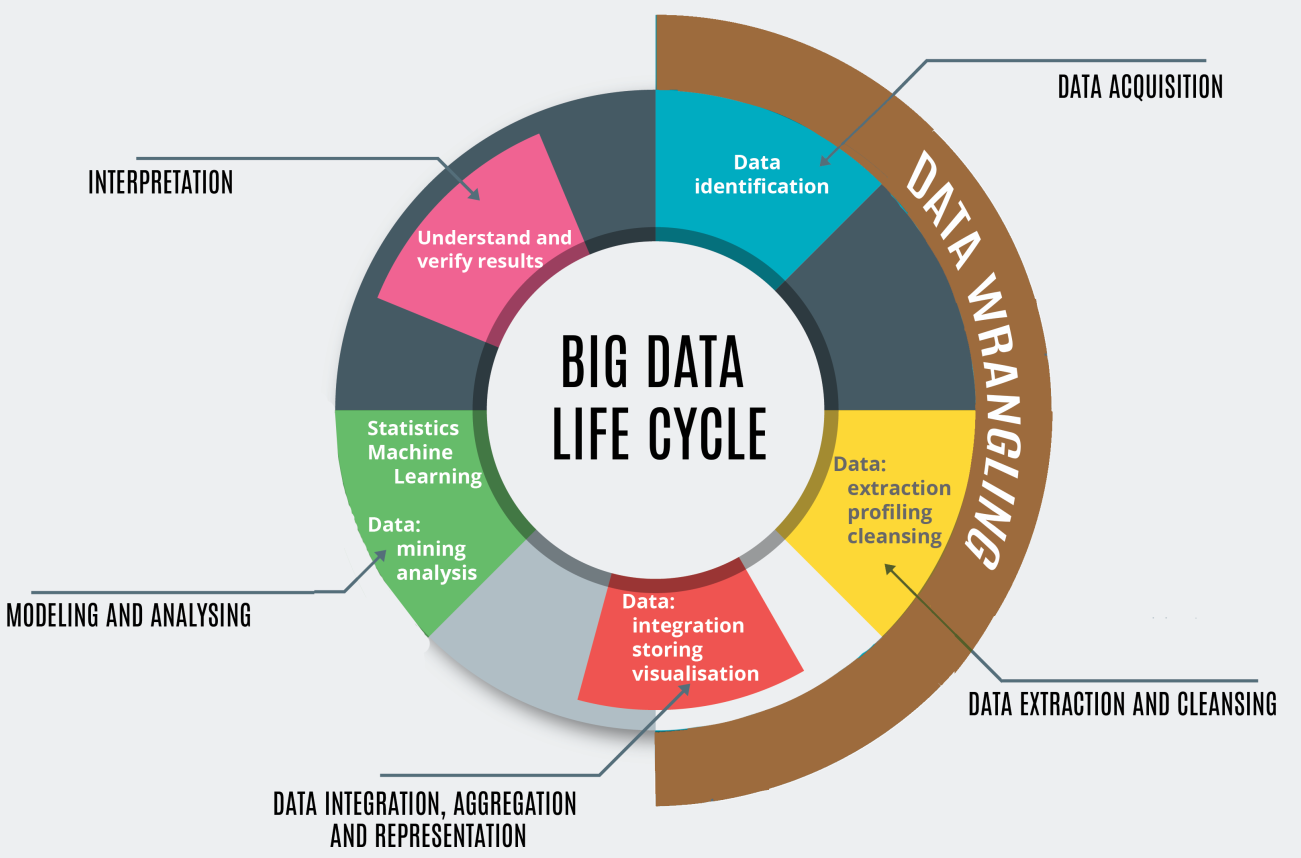
\includegraphics[scale=.3]{big_data_life_cycle}
	\caption{The big data life cycle}
	\label{fig:img_big_data_life_cycle}
\end{figure}


\begin{table}[H]
	\caption{Big data life cycle processes definitions I.}
	\label{table:big_data_life_cyle_processes_definition_I}
	\centering
	\begin{tabular}{p{4.0cm} p{3.1cm} p{7cm}}
		\toprule
		\textbf{Major Process} & \textbf{Process included} & \textbf{Description} \\ 
		\bottomrule
		DATA ACQUISITION & Data identification & Data has to be first generated from the
		real world, then converted to electrical signals so it can then be recorded
		in a machine. This process is called data acquisition  ~\cite{ComputingResearchAssociation}. Identifying
		data means to provide useful metadata about its provenance, intended use, recording place and motivation,
		etc. ~\cite{Dataone2016} ~\cite{Microsoft2016}. \\
		DATA EXTRACTION AND CLEANSING &  Data extraction & This is the process in which data from
		source systems is selected and transformed into a suitable type of data according to its purpose, e.g. coordinates from a set of stored satellite images ~\cite{ComputingResearchAssociation}.    
		\\
		& \\ &  Data profiling & This refers to generating convenient metadata to 
		support measurements against quality settings previously established, and to contribute towards
		“well known data”, clearing up the structure, content and/or relationships among the data. E.g. data types,data domains, timeliness, completeness, statistics, etc.~\cite{Sandra2015} ~\cite{Kimball2008}.
		\\
		& \\ & Data cleansing & Also known as cleaning or scrubbing.
		Requires solving errors found in invalid, inconsistent, incomplete or duplicated data so the quality of the data
		can be improved. To find the errors this process relies on profiling information ~\cite{Sandra2015} ~\cite{Erhard2000}.
		\\ 
		DATA INTEGRATION, AGGREGATION AND REPRESENTATION & Data integration & Integrating data involves combining data from multiple sources into one,
		meaningful and valuable set of data ~\cite{Lenzerini2002} ~\cite{Halevy2006} ~\cite{Sandra2015}.
		\\
		\bottomrule
	\end{tabular}
\end{table}

\begin{table}[H]
	\caption{Big data life cycle processes definitions II.}
	\label{table:big_data_life_cyle_processes_definition_II}
	\centering
	\begin{tabular}{p{4.0cm} p{3.1cm} p{7cm}}
		\toprule
		\textbf{Major Process} & \textbf{Process included} & \textbf{Description} \\ 
		\bottomrule   
		& \\ &  Data storing & To preserve integrated data understandable, maintaining its quality, and
		adequacy to its purpose, it is also required to develop a suitable storage
		architecture design, taking into account the type of database suitableness (e.g. relational, non-relational),
		the capacities of the database management system, etc., among all the alternatives in which data could be stored. ~\cite{ComputingResearchAssociation}
		\\
		& \\ & Data visualization & Typically one step before analysis
		techniques. This process is about applying a graphical representation to
		the data, aimed at providing ease at future usage, transformation and understanding ~\cite{Fayyad2002} ~\cite{Ware2012} ~\cite{Philip2014}.
		\\ 
		MODELING ANALYZING & Statistics \&\ machine learning & This concerns about stating facts in
		this context, from a given dataset, by interpreting data and providing a numerical picture of it, as well as using computer systems that emulate the human learning process, saving new information and outcomes,
		closely related to artificial intelligence (AI). Parallel statistics algorithms have been proposed to approach big data ~\cite{Ryszard2013}~\cite{PhilipChen2014}.
		\\
		& \\ & Data mining & This process involves techniques to
		find latent valuable information, revealing patterns, cause-effect relations, implicit facts, etc., to hold up
		data analysis ~\cite{Chandrasekar2001} ~\cite{Philip2014} .
		\\
		\bottomrule
	\end{tabular}
\end{table}

\begin{table}[H]
	\caption{Big data life cycle processes definitions III.}
	\label{table:big_data_life_cyle_processes_definition_III}
	\centering
	\begin{tabular}{p{4.0cm} p{3.1cm} p{7cm}}
		\toprule
		\textbf{Major Process} & \textbf{Process included} & \textbf{Description} \\ 
		\bottomrule   
		& \\ & Data analysis & A task done by the perceptual and
		cognitive system of an analyst, although nowadays machine learning
		and AI techniques can also be used. This is the ultimate phase in the process of obtaining the value from the
		data, by finding the significance on the insights provided by, for example,
		correlations or graphical representations. ~\cite{Ware2012}
		\\
		INTERPRETATION & Understand and verify results & This is the phase in which the information obtained is used and trans-
		formed into a decision that could lead
		to a tangible value (e.g. economic gaining, marketing advantages, scientific progress ), differing each time
		according to the context on which it has been obtained and its purpose This phase also comprises retracing
		the results obtained, verifying them and testing them in several use cases
		~\cite{ComputingResearchAssociation}.
		\\
		\bottomrule
	\end{tabular}
\end{table}

In order to support the value characteristic of the data it is important to satisfy
high quality conditions of the large data sets ~\cite{ZhuCai2015}, where quality could be measured
by its dimensions, having completeness, uniqueness, timeliness, validity, accuracy and
consistency considered as the six core ones ~\cite{DAMA2013}, among other identified dimensions,
such as reputation, security, transactability, accesibility and interpretability ~\cite{Pipino2002} ~\cite{McGilvary2008}.
The processes, technologies and techniques aimed at obtaining the value from big
data, are known as big data analytics ~\cite{Kwon2014}, applied in several ambits, such as health
care, social sciences, environmental and natural resources area, business and economic
domains, and technology fields. Recently, big data quality has been approached from a
big data analytics point of view ~\cite{Kambatla2014} ~\cite{Hazen2014} ~\cite{Lavalle2011}. Some studies might conclude that data
quality is not a bigger challenge than the lack of knowledge from analysts to implement 

the correct methods to manage big data value ~\cite{Lavalle2011}, however, data management is an
inherent phase of the big data analytics, and it involves the capacity to gather, integrate
and analyze data as well, where data quality should not be considered as a separate
phase.
The Data Warehousing Institute estimated low quality data cost U.S. businesses
more than 600 billion USD per annum ~\cite{Eckerson2002}. The U.S. Postal Service estimated that
wrong data cost 1.5 billion USD in 2013 from mailpieces that could not been delivered
to the given addresses, facing data quality problems from around 158 billion mailpieces
in that single year. Data quality management strategies were recommended to increase
address information accuracy, timeliness and completeness ~\cite{USAPostService2014}. In big data, “low”
error rates translate into millions of faults annually, where the risk is to lose 10-25\%\ of
the total revenues from it ~\cite{Eckerson2002}.
Big data quality requires multidisciplinary participation to progress ~\cite{Hazen2014} and propel the development of simple and low-cost data quality techniques, reduce the cost of
poor quality data, the data error rate, and the need of data cleansing processes which
involve investing not only budget, but time and effort to manage. IS research is demanded to collaborate with data wrangling insights and advances, working together
with statistical experts to leverage the techniques involved, where domain specific authorities are needed to set the data analytics management, which should support the
right value retrieval out of relevant problems from each area ~\cite{Hazen2014}.

\section{The Concept of Data Quality}

From a research perspective, data quality has been addressed in different
areas, including statistics, management, and computer science. Statisticians were the first to investigate some of the problems related to data quality, by
proposing a mathematical theory for considering duplicates in statistical data sets, in the late 1960's. They were followed by researchers in management, who
at the beginning of the 1980's focused on how to control data manufacturing systems in order to detect and eliminate data quality problems. Only at the
beginning of the 1990's computer scientists begin considering the problem of defining, measuring, and improving the quality of electronic data stored in
databases, data warehouses, and legacy systems.

Dr. Genichi Taguchi~\citep{Jugulum14}, who was a world-renowned quality engineering expert from Japan, emphasized and established the relationship between
poor quality and overall loss. Dr. Taguchi (1987) used a quality loss function (QLF) to measure the loss associated with quality characteristics
or parameters. The QLF describes the losses that a system suffers from an adjustable characteristic. According to the QLF, the loss increases as
the characteristic y (such as thickness or strength) gets further from the target value (m). In other words, there is a loss associated if the quality
characteristic diverges from the target. Taguchi regards this loss as a loss to society, and somebody must pay for this loss. The results of such losses
include system breakdowns, company failures, company bankruptcies, and so forth.

Figure 1.1 shows how the loss arising from varying (on either side)
from the target by $\Delta_0$ increases and is given by $L(y)$ when $y$ is equal to $m$,

\begin{figure}[htbp!] 
\centering    
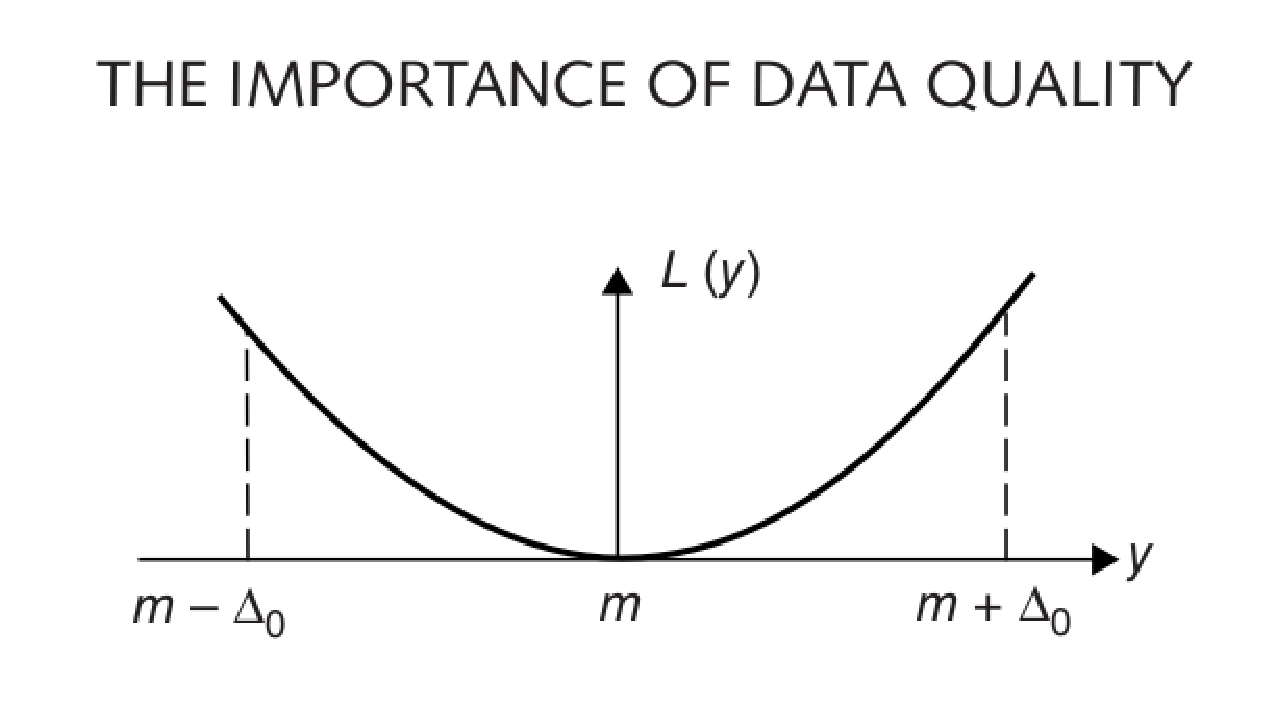
\includegraphics[width=0.6\textwidth]{quality-loss-function}
\caption{Quality Loss Function (QLF)}
\end{figure}

the loss is zero, or at the minimum. The equation for the loss function can
be expressed as follows:

\begin{equation*}
    L(y) = k(y-m)^2
\end{equation*}

where $k$ is a factor that is expressed in dollars, based on direct costs, indirect costs, 
warranty costs, reputational costs, loss due to lost customers,
and costs associated with rework and rejection. There are prescribed ways
to determine the value of $k$.
The loss function is usually not symmetrical-sometimes it is steep on
one side or on both sides. Deming ~\citep{Deming} says that the loss function need
not be exact and that it is difficult to obtain the exact function. As most
cost calculations are based on estimations or predictions, an approximate
function is sufficient-that is, close approximation is good enough.

The concept of the loss function aptly applies in the DQ context, especially when we are measuring data quality associated with various data
elements such as customer IDs, social security numbers, and account balances. Usually, the data elements are prioritized based on certain criteria,
and the quality levels for data elements are measured in terms of percent-
ages (of accuracy, completeness, etc.). The prioritized data elements are
referred to as critical data elements (CDEs).


\section{The Specificity of DQ in Big Data}

The term big data itself comprises a deeper meaning, being not only a term to be
defined but the name of a phenomenon and an emerging discipline ~\cite{Diebold2012}. 
The earliest mentions of big data were made, to the best of my knowledge, in 1979 by Lawrence
Stone, when describing the work of cliometricians dealing with “vast quantities of data
using electronic computers to process it and applying mathematical procedures” ~\cite{Lawrence1979},
and by Charles Tilly, who in 1980 describing the work done by the former, used the
term “big-data people” referring to the cliometricians Stone mentioned before ~\cite{Tilly1980}.
Then, in 1997 Michael Cox and David Ellsworth, described the term as large data
sets that surpasses the available size in main memory, local disk and even remote disk
~\cite{Cox1997}. Following that year, Sholom M. Weiss and Nitin Indurkhya in their book “Predictive data mining: a practical guide”, contextualize not only the term but the phenomenon, 
mentioning that “millions or even hundreds of millions of individual records can lead to much stronger conclusions, making use of powerful methods to examine
data more comprehensively” and also acknowledges that analyzing big data, in practice, has many difficulties ~\cite{Sholom1998}. Two years later, Francis X. Diebold defined big data
as “the explosion in the quantity of available and potentially relevant data, largely the
result of recent and unprecedented advancements in data recording and storage technology”. By this time, it was clear that big data was not only about size, but about
the insights that a large set of data could eventually bring.

The Oxford English Dictionary, which added the term to its data base in 2013
~\cite{OxfordDictionaries2013}, defines big data as “data of a very large size, typically to the extent that its
manipulation and management present significant logistical challenges”.

Nevertheless, those “logistical challenges” for one organization could be necessary
to be done when facing a smaller size of data compared to another ~\cite{Magoulas2009}, in this sense, it seemed that relying only in the size depends on the available technology within each organization and its capability to handle a given amount of data, so, to scope the definition, the size of big data could be thought as the size in which using traditional
techniques to process it, is not longer an option. 

The above led to define big data not only regarding size, but taking into account
another identified characteristics, known as the “V’s of big data” ~\cite{Marr2015} : Volume, Velocity, Variety, Veracity and Value; where Volume refers to the data size, 
Velocity evokes the high speed of change and fast generation of data, Variety relates to the different type of data (structured, unstructured and semistructured), 
Veracity is the degree of trustworthiness of the data (quality and accuracy) and Value indicates the
worth or benefit of gathering, storing, processing and analyzing the data.

Because of the nature of big data, traditional approaches to managing data are not
suitable, for example, since the main aim was to handle relational data, and as previously mentioned,  big data is not always relational, so, traditional techniques are not expected to work correctly ~\cite{FUJITSU2015}. 

When processing data, one of the main challenges faced with big data is the large volume of it; this require scaling, and there have been two types of scaling for big data processing: scaling-up and scaling-out, where the former is about implementing powerful machines, with great memory and storage capacity, as well as quick but expensive processors, and the latter refers to the usage of several commodity machines connected as clusters, having a parallel environment, suitable to handle large volumes of data, and an advantageous price-performance relation, compared to the scaling-up approach [88] ~\cite{FUJITSU2015}. For big data frameworks, it is known that with the proper optimizations, scaling-up performs better than scaling-out ~\cite{Appuswamy2013}, however, it is still unknown exactly when is better to opt for one approach or the other,
this is, the results presented were not dependable on the framework solely, but on the
processed data characteristics. Nevertheless, it might be strongly preferred to utilize
several smaller machines than high performance computer systems (HPC), because of
the higher cost scaling-up represents, and considering the support that new paradigms
provide by avoiding the necessity to communicate data, but having the processing ap-publications running where the data is, which proposes a significant performance advantage ~\cite{Tekiner2013}, trading off performance in certain degree for a better cost-benefit ratio.


\section{Why Data Quality is Relevant}

The consequences of poor quality of data are often experienced in everyday life, but often, without making the necessary connections to their causes.

For example, the late or mistaken delivery of a letter is often blamed on a postal service, although  a closer look often reveals data-related causes, typically an error in the address, originating in the address database.

Data quality has serious consequences of far-reaching significance, for the efficiency and effectiveness of organizations and business.



\section{Why Data Quality is Matters}

Poor data quality is enemy number one to the widespread, profitable use of machine learning. While the caustic observation, “garbage-in, garbage-out” has plagued analytics and decision-making for generations, it carries a special warning for machine learning. The quality demands of machine learning are steep, 
and bad data can rear its ugly head twice - first in the historical data used to train the predictive model and second in the new data used by that model to make future decisions. ~\cite{RedmanHBR2018}

Data quality is no less troublesome in implementation. Consider an organization seeking productivity gains with its machine learning program. While the data science team that developed the predictive model may have done a solid job cleaning the training data, it can still be compromised by bad data going forward. Again, it takes people — lots of them — to find and correct the errors. This in turns subverts the hoped-for productivity gains. Further, as machine learning technologies penetrate organizations, 
the output of one predictive model will feed the next, and the next, and so on, even crossing company boundaries. The risk is that a minor error at one step will cascade, causing more errors and growing ever larger across an entire process.

Bad data costs the U.S. \$3 trillion per year, IBM’s estimate of the yearly cost of poor quality data, in the US alone, in 2016. While most people who deal in data every day know that bad data is costly, this figure stuns. ~\cite{ibmInfoGraphic}


Importantly, the benefits of improving data quality go far beyond reduced costs. It is hard to imagine any sort of future in data when so much is so bad. Thus, improving data quality is a gift that keeps giving — it enables you to take out costs permanently and to more easily pursue other data strategies. 
For all but a few, there is no better opportunity in data.

\begin{figure}[H]
    \centering
    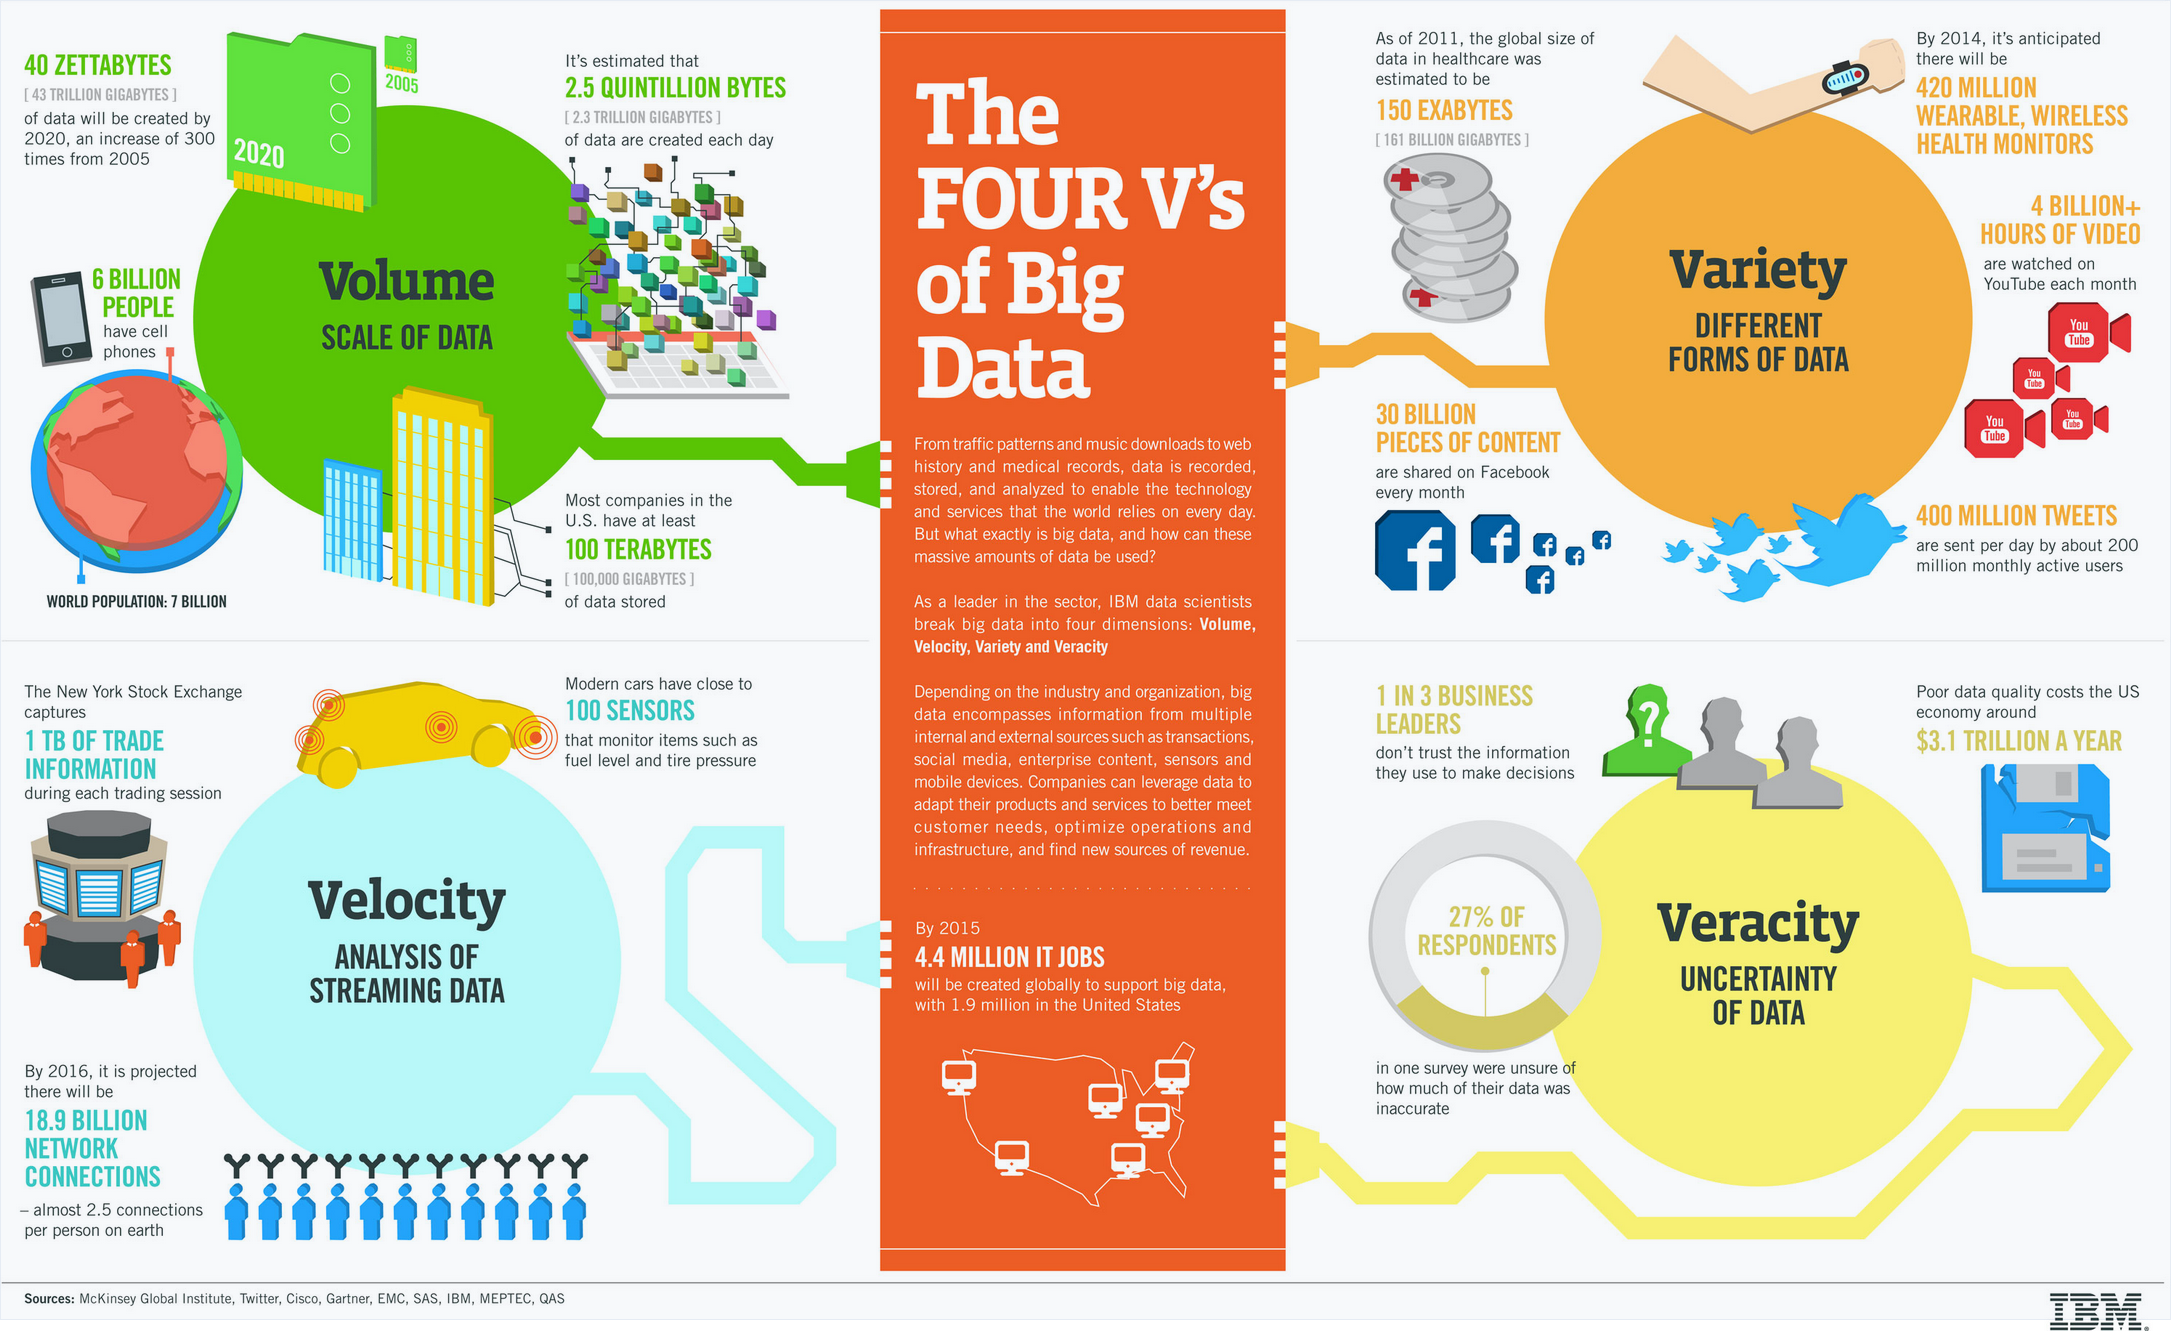
\includegraphics[angle=-90,scale=.3]{4-Vs-of-big-data}
    \caption{IBM data scientists break big data into four dimensions: volume, variety, velocity and veracity. This infographic explains and gives examples of each. ~\cite{ibmInfoGraphic}}
\end{figure}

\section{Data Quality and Types of Information Systems}

Data are collected, stored, elaborated, retrieved, and exchanged in information systems used in organizations to provide services to business processes.
Different criteria can be adopted for classifying the different types of information systems, and their corresponding architectures; they are usually related to
the overall organizational model adopted by the organization or the set of the
organizations that make use of the information system.

The three classifications are represented together in the classification space of Figure 1.2.
Among all possible combinations, five main types of information systems are highlighted in the figure:
Monolithic, Distributed, Data Warehouses,Cooperative, and Peer-to-Peer.


\begin{itemize}
    \item{In a \textit{monolithic information system} presentation, application logic, and data management are merged into a single computational node.
    Many monolithic information systems are still in use. While being extremely rigid, they provide advantages to organizations, such as reduced costs due to homogenetiy of solutions and centralization of management.
    In monolithic systems data flows have a common format, and data quality control is facilitated by the homogenetiy and centralization of procedures and management rules.}
    \item {A \textit{data warehouse} (DW) is a centralized set of data collected from different sources, designed to support management decision making. The most critical problem in DW design concerns the cleaning and integration of 
    the different data sources that are loaded into the DW, in that much of the implementation budget is spent on data cleaning activities.}
    \item{A \textit{distributed information system} relaxes the rigid centralization of monolithic systems, in that it allows the distribution of resources and applications across
    network of geographically distributed systems.
    The network can be organized in terms of several tiers, each made of one or more computational nodes. Presentation, application logic, and data management are distributed across tiers. Usually, the different tiers and nodes have a limited degree of autonomy, 
    data design is usually performed centrally, but to a certain extent some degree of heterogenetiy can occur, due to the impossibility of establishing unified procedures.
    Problems of data management are more complex than in monolithic systems, due to the reduced level of centralization.
    }  
\end{itemize}

\begin{figure}[H]
% \vspace*{.0in}
\centering
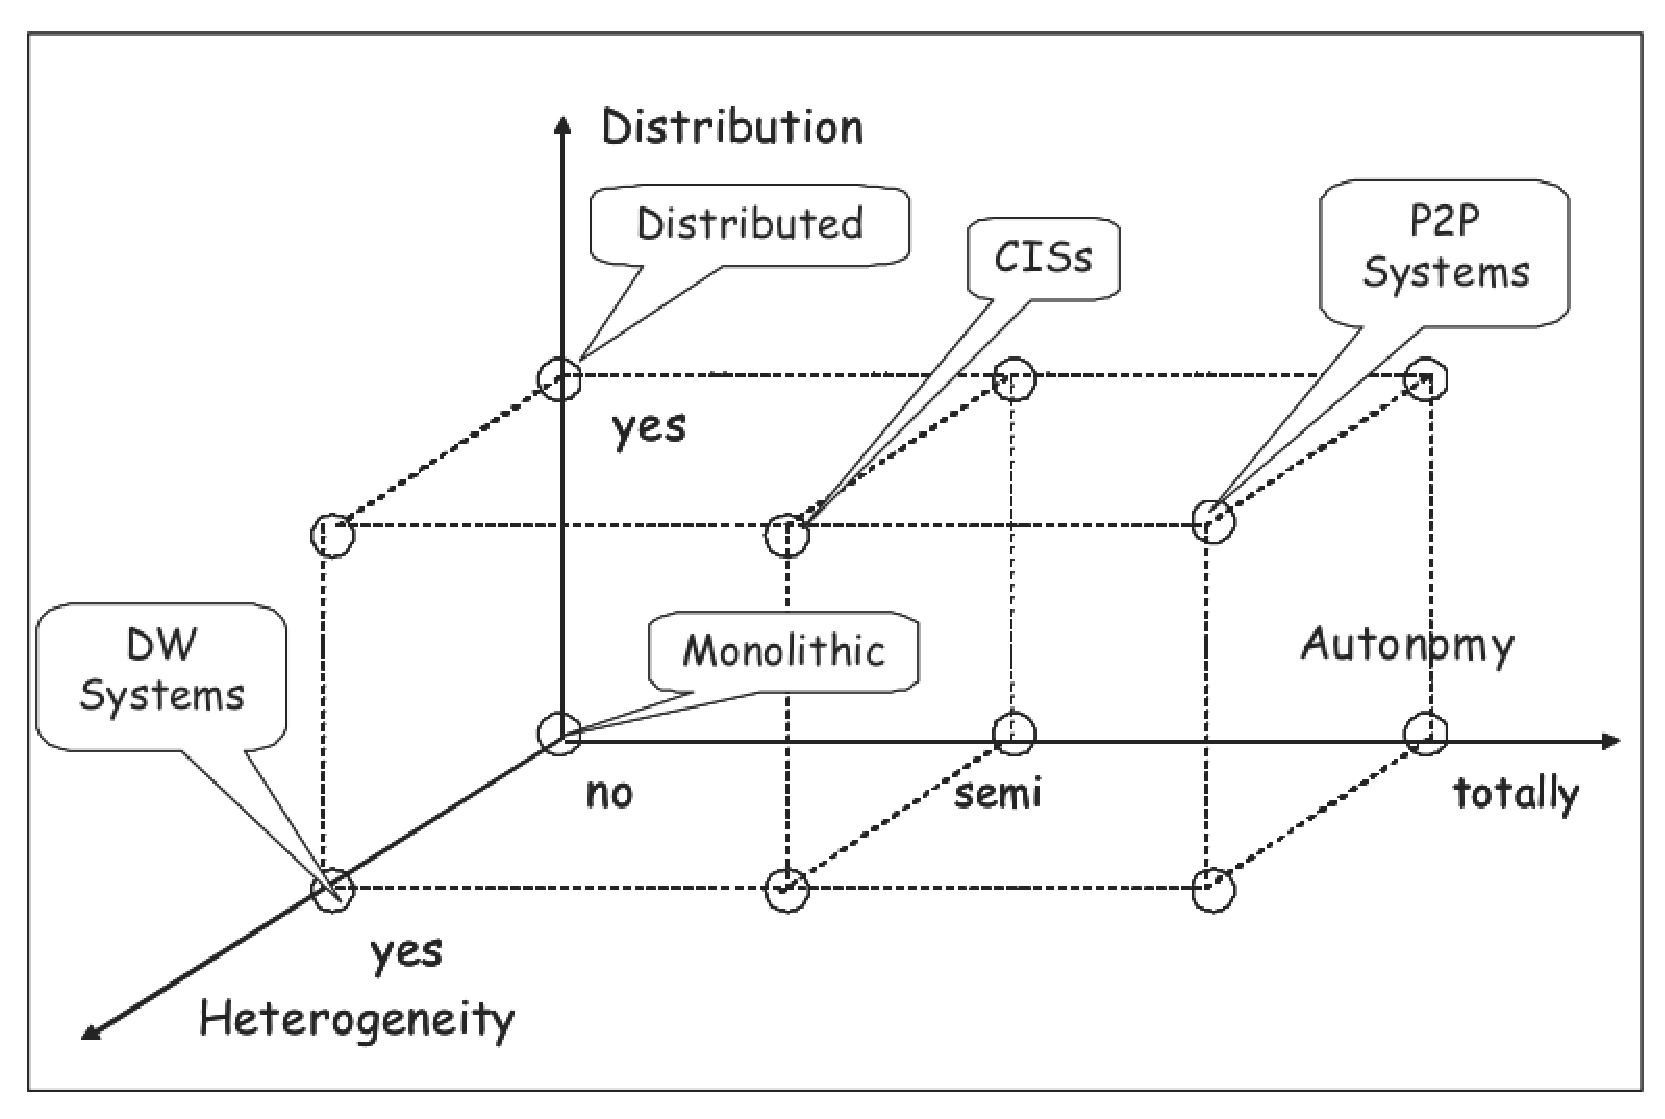
\includegraphics[scale=.50]{types-of-information-systems}
\caption{Types of information systems}    
\end{figure}

\begin{itemize}
    \item{A \textit{coorparative information system} (CIS) can be defined as a large-scale information system that interconnects various systems of different and autonomous organizations, 
    while sharing common objectives.}
    \item{In a \textit{peer to peer information system} (usually abbreviated P2P), the traditional distinction between clients and servers typical of distributed systems is disappearing.
    A P2P system can be characterized by a number of properties: peers are highly autonomous and highly heterogeneous, they have no obligation for the quality of their services
    and data, no central coordination and no central database exist, no peer has a global view of the system, global behavior emerges from local intreactions.    
    }
\end{itemize}


\section{Main Research Issues and Application Domains in Data Quality}
Due to the relevance of data quality, its nature, and the variety of data types and information systems, achieving data quality is a complex, multidisciplinary 
area of investigation. I involves several research topics and real-life application areas

\begin{figure}[H]
%\vspace*{.0in}
\centering
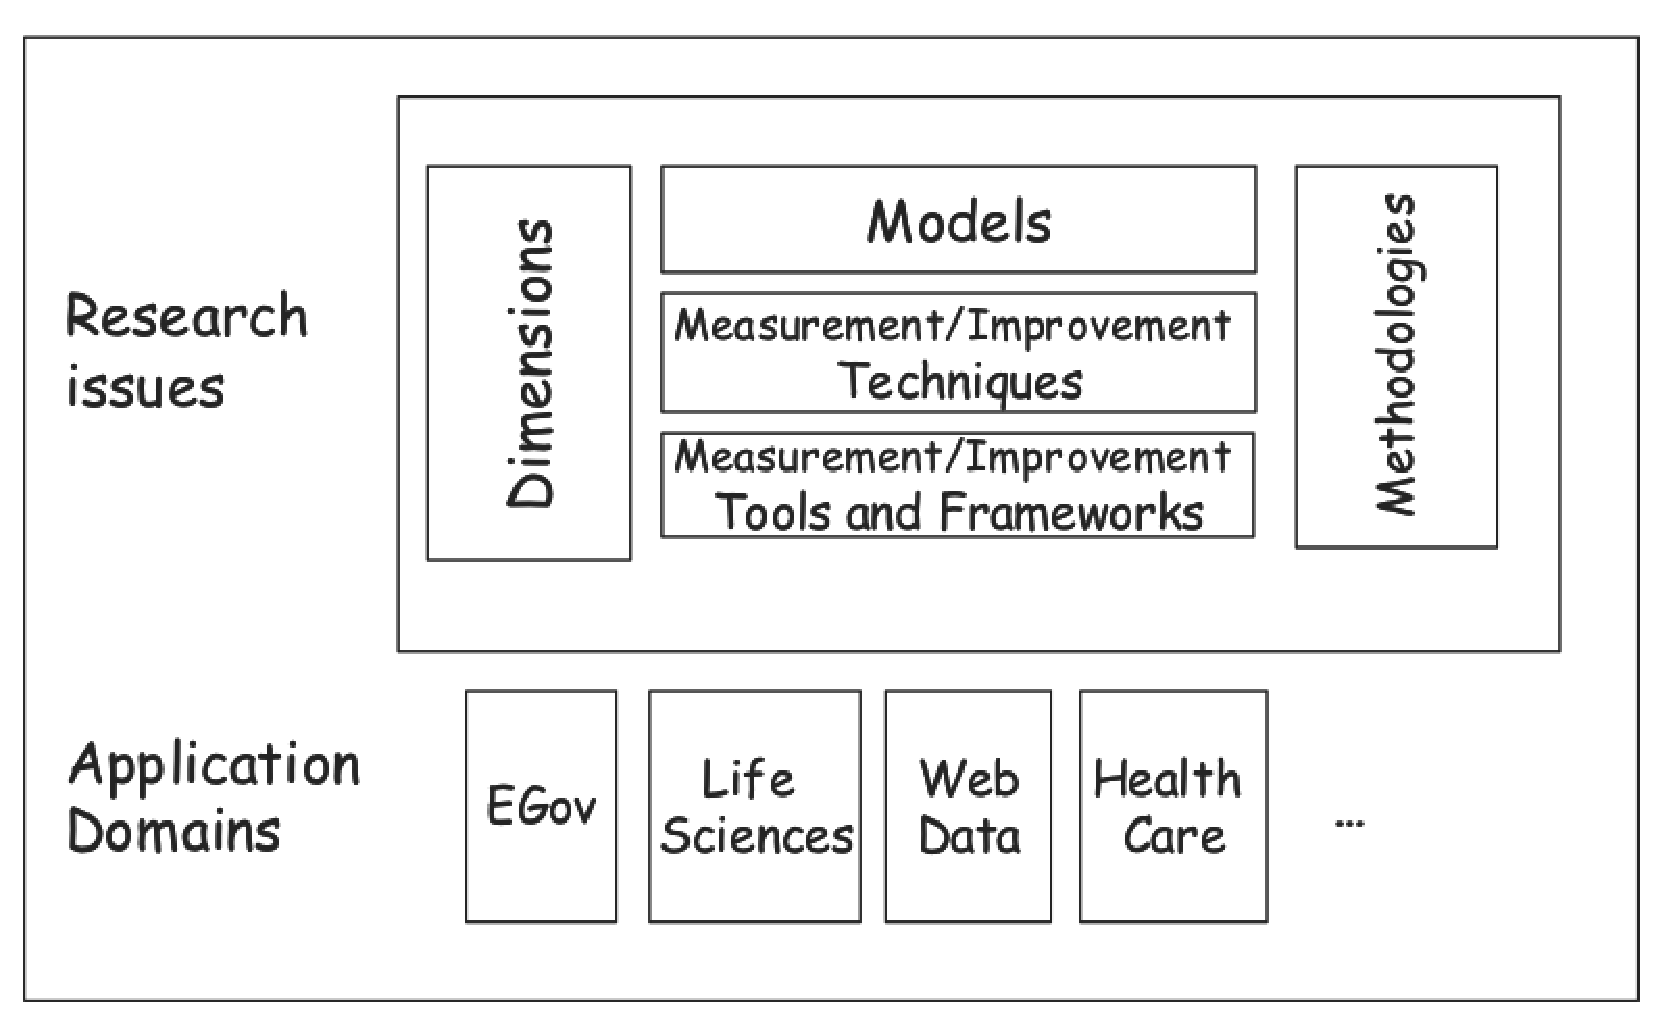
\includegraphics[scale=.50]{main-issues-in-dq}
\caption{Main issues in data quality}    
\end{figure}
%!TEX root = ../thesis.tex
%*******************************************************************************
%****************************** Second Chapter *********************************
%*******************************************************************************
\chapter{Data Quality Dimensions}

\ifpdf
    \graphicspath{{Chapter2/Figs/Raster/}{Chapter2/Figs/PDF/}{Chapter2/Figs/}}
\else
    \graphicspath{{Chapter2/Figs/Vector/}{Chapter2/Figs/}}
\fi

More specifically, quality dimensions can refer either to the extension of data, i.e., to data values, or to their 
intension, i.e., to their schema. Both data dimensions are usually defined in qualitative way, referring to general properties of data and schemas,
and and related definitions do not provide any facility for assigning values to dimensions themselves. 

Specifically, definitions do not provide quantitative measures, and one or more metrics are to be associated with dimensions as separate, distinct 
properties. For each metric, one or more measurement metadata are to be provided regarding (i) where the measurement is taken, (ii) what data are included, 
(iii) the measurement device, and (iv) the scale on which results are reported.

According to the literature, at times we will distinguish between dimensions and metrics, while other times we will directly metrics.

\begin{table}[H]
\caption{Data Quality Dimensions I}
\centering
\begin{tabular}{p{4.0cm} p{10cm}}
\toprule
\textbf{Dimension Name} & \textbf{Description} \\ 
\bottomrule
Data Governance & 
Do organization-wide data standards exist and are they enforced? Do clearly
defined roles and responsibilities exist for data quality related activities? Does
data governance strive to acquire and maintain high-quality data through proactive
management? \\
Data Specifications &
Are data standards documented in the form of a data dictionary, 
data models, meta data, and integrity constraints?  
\\
Data Integrity & 
How is data integrity maintained? How are data integrity violations detected and
resolved ?   
\\
Data Consistency & 
If data redundancy exists, how is data consistency achieved? What methods
are used to bring consistency to data that has become inconsistent? If data is
geographically replicated, how is the consistency and latency managed? 
\\
Data Currency & 
Is the data current? Do procedures exists to keep the data current and purge stale
data? 
\\
Data Duplication & Are there effective procedures in place to detect and remove duplicate data? 
\\
Data Completeness & 
Is the data about entities complete? How is missing data managed? 
\\
Data Provenance & 
Is a historical record of data and its origination maintained? If the data is acquired
through multiple sources and has undergone cleaning and transformations, does
the organization maintain a history of all changes to the data? 
\\
Data Heterogeneity & 
If multi-modality data about an entity is available, is that data captured and used? 
\\
Streaming Data & 
How is streaming data sampled, filtered, stored, and managed for both real-time
and batch processing? 
\\
Outliers & 
How are outliers detected and addressed? Are there versions of datasets that
are outlier-free? Does each version correspond to a different method for outlier
detection and treatment? 
\\
Dimensionality &
Reduction Do the datasets feature dimensionality reduced versions? How many versions are
available? \\
Feature Selection & 
Do datasets have versions that exclude features that are either redundant, highly
correlated, or irrelevant? How many versions are available? 
\\
\bottomrule
\end{tabular}
\end{table}

\begin{table}
% \vspace*{-3.5in}
\caption{Data Quality Dimensions II}
\centering
\begin{tabular}{p{4.0cm} p{10cm}}
\toprule
\textbf{Dimension Name} & \textbf{Description} \\ 
\bottomrule
Feature Extraction & 
Do the datasets provide a set of derived features that are informative and non-
redundant, in addition to the original set of variables/features? How many such
derived feature sets are available? 
\\
Business Rules & 
Does a process exist to identify, refine, consolidate, and maintain business
rules that pertain to data quality? Do rules exist to govern data cleaning and
transformations, and integrating related data of an entity from multiple sources?
What business rules govern substitutions for missing data, deleting duplicate data,
and archiving historical data? Are there rules for internal data audit and regulatory
compliance? \\
Data Accuracy & 
Data can be syntactically accurate and yet semantically inaccurate. For example,
a customer's mailing address may meet all the syntactic patterns specified by the
postal service, yet it can be inaccurate. How does the organization establish the
accuracy of data? \\
Gender Bias & 
Is the data free from factors that lead to gender bias in machine learning
algorithms? \\
Confidentiality and Privacy & 
Are procedures and controls implemented for data encryption, data de-
identification and re-identification, and differential privacy? \\
Availability and Access Controls & 
How is high data availability achieved? What security controls are implemented to
protect data from unauthorized access? How are user entitlements to data access
and modifications defined and implemented? \\
\bottomrule
\end{tabular}
\end{table}


\section{Accuracy}

Accuracy ~\citep{Falorsi} is defined as the closeness between a value v and a value v' , considered as 
the correct representation of the real-life phenomenon that v aims to
represent. As an example if the name of a person is Ayta?, the value v' = Ayta?
is correct, while the value v = Ayt is incorrect. Two kinds of accuracy can be
identified, namely a syntactic accuracy and a semantic accuracy.

Let us consider a relation schema \textbf{R} consisting of \textbf{K}
attributes and a relational table \textbf{r} consisting of N tuples. 

Let $q_{ij}(i=1..N, j=1..K)$ be a boolean variable defined to correspond to the cell values 
$y_{ij}$, is syntactically accurate, while otherwise it is equal to 1. 

In order to identify whether or not accuracy errors affect a matching of 
relational table \textbf{r} with a reference table \textbf{r'} containing correct
values, we introduce a further boolean variable $s_i$ equal to 0 if the tuple $t_i$ 
matches a tuple in \textbf{r'}, and otherwise equal to 1. We can introduce three metrics to distinguish
the relative importance of value accuracy in context of the tuple.
The first two metrics have the purpose of giving a different importance to 
errors on attributes that have a higher identification power, in line with 
the above discussion.

The first metric called \textit{weak accuracy error,} and is defined:

\begin{equation*}
    \sum_{i = 1}^{N} \frac{\beta(q_i > 0)\wedge(s_i=0)}{N}
\end{equation*}

where $\beta(.)$ is a boolean variable equal to 1 if the condition in parentheses is 
\textit{true}, 0 otherwise, and $q_i =\sum\nolimits_{j=1}^K q_{ij}$. Such metric considers the case in 
which for a tuple $t_i$ accuracy errors occur $(q_i > 0)$ but do not affect identification
$(s_i = 0)$.

The second metric is called \textit{strong accuracy error}, and is defined assigning

\begin{equation*}
    \sum_{i = 1}^{N} \frac{\beta(q_i > 0)\wedge(s_i=1)}{N}
\end{equation*}

where $\beta(.)$ and $q_i$ have the same meaning as above. Such a metric considers
the case which accuracy errors occur $(q_i > 0)$ for a tuple $t_i$ and actually 
do affect identification $(s_i = 1)$.

The third metric gives the percentage of accurate tuples matched with
the reference table. It is expressed by the degree of syntactic accuracy of the
relational instance \textbf{r}

\begin{equation*}
    \sum_{i = 1}^{N} \frac{\beta(q_i =0)\wedge(s_i=0)}{N}
\end{equation*}

by actually considering the fraction of accurate $(q_i = 0)$ matched $(s_i =0)$ tuples.

\section{Completeness}
Completeness can be generically defined as the extent to which data are
of sufficient breadth, depth, and scope for the task at hand ~\cite{Wang}
three types of completeness are identified. Schema completeness is defined as
the degree to which concepts and their properties are not missing from the
schema. Column completeness is defined as a measure of the missing values for
a specific property or column in a table. Population completeness evaluates
missing values with respect to a reference population.
If focusing on a specific data model, a more precise characterization of
completeness can be given. In the following we refer to the relational model.

\subsection{Completeness of Web Data}

Data that are published in Web information systems can be characterized by
evolution in time. While in the traditional paper-based media, information
is published once and for all, Web information systems are characterized by
information that is continuously published.

We consider a function $C(t)$, defined as the value of completeness at the
instant \textit{t}, with $t\in$ $[t\_pub, t\_max]$ , where t pub is the initial 
instant of publication of data and ${t\_max}$ corresponds to the maximum time within which the
series of the different scheduled updates will be completed. Starting from the
function $C(t)$, we can define the completability of the published data as

\begin{equation*}
    \int\nolimits_{t\_curr}^{t\_max} C(t),
\end{equation*}

where ${t\_curr}$ is the time at which completability is evaluated and ${t\_curr}$ <
${t\_max}$.

Completability, as shown in Figure 2.1, can be graphically depicted as an
area Cb of a function that represents how completeness evolves between an
instant ${t\_curr}$ of observation and t max. Observe that the value corresponding
to ${t\_curr}$ is indicated as ${c\_curr}$; ${c\_max}$ is the value for completeness estimated
for t max. The value ${c\_max}$ is a real reachable limit that can be specified for
the completeness of the series of elements; if this real limit does not exist,
${c\_max}$ is equal to 1. In Figure 2.5, a reference area A is also shown, defined as

\begin{equation*}
    ({t\_max}-{t\_curr}) * \frac{{c\_max - {c\_pub}}}{2},
\end{equation*}

that, by comparison with Cb, allows us to define ranges [High, Medium, Low]
for completability.

\begin{figure}[H]
    \vspace*{.0in}
    \centering
    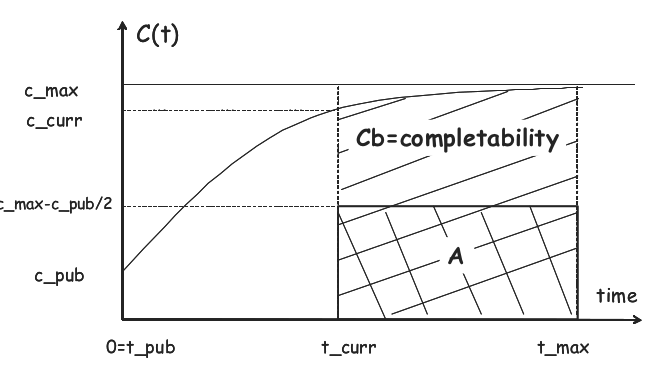
\includegraphics[scale=.50]{completeness_of_web_data}
    \caption{A graphical representation of completability}    
\end{figure}

With respect to the example above, considering the list of courses published on a university Web site, the completeness dimension gives information
about the current degree of completeness; the completability information gives
the information about how fast this degree will grow in time, i.e., how fast
the list of courses will be completed. The interested reader can find further
details in ~\cite{pernicib.scannapiecom.2003}.

\section{Consistency}

The consistency dimension captures the violation of semantic rules defined
over (a set of) data items, where items can be tuples of relational tables or
records in a file. With reference to relational theory, integrity constraints are
an instantiation of such semantic rules. In statistics, data edits are another
example of semantic rules that allow for the checking of consistency.

\subsection{Integrity Constraints}
Integrity constraints are properties that must be satisfied by all instances
of a database schema. Although integrity constraints are typically defined on
schemas, they can at the same time be checked on a specific instance of the
schema that presently represents the extension of the database. Therefore,
we may define integrity constraints for schemas, describing a schema quality
dimension, and for instances, representing a data dimension.

Most of the considered integrity constraints are dependencies. The following main types of dependencies can be considered:

\begin{itemize}
    \item{\textit{Key Dependency.} This is the simplest type of dependency. Given a relation
    instance r, defined over a set of attributes, we say that for a subset K of
    the attributes a key dependency holds in r, if no two rows of r have the
    same K-values. For instance, an attribute like SocialSecurityNumber can
    serve as a key in any relation instance of a relation schema Person.}
    \item{\textit{Inclusion Dependency.} Inclusion dependency is a very common type of
    constraint, and is also known as referential constraint. An inclusion de-
    pendency over a relational instance r states that some columns of r are
    contained in other columns of r or in the instances of another relational in-
    stance s. A foreign key constraint is an example of inclusion dependency,
    stating that the referring columns in one relation must be contained in the
    primary key columns of the referenced relation.}
    \item{\textit{Functional Dependency.} Given a relational instance \textbf{r}, let \textbf{X} and \textbf{Y} be two
    nonempty sets of attributes in \textbf{r}. \textbf{r} satisfies the functional dependency
    ${\textbf{X} \rightarrow \textbf{Y}}$ if the following holds for every pair of tuples \textbf{$t_1$} and \textbf{$t_2$} in \textbf{r}:
    }
\end{itemize}

\begin{equation*}
    \boxed{If, t_1.X = t_2.X, then, t_1.Y = t_2.Y,}
\end{equation*}

where the notation $t_1.X$ means the projection of the tuple $t_1$ onto the
attributes in $X$.

\section{Other Data Quality Dimensions}
There are general proposals for sets of dimensions that aim to fully specify
the data quality concept in a general setting Some other
proposals are related to specific domains that need ad hoc dimensions in order
to capture the peculiarities of the domain. For instance, specific data quality
dimensions are proposed in the following domains:

\begin{enumerate}
    \item {The archival domain (see ~\cite{wiszniewskib.krawczykh.2003} and ~\cite{krawczykh.wiszniewskib.2003})
    which makes use of dimensions such as condition (of a document) that
    refers to the physical suitability of the document for scanning.}
    \item {The statistical domain; every National bureau of census and international
organizations such as the European Union or the International Monetary Fund define several dimensions for statistical and scientific data,
such as integrity, on the notion that statistical systems should be based on adherence to the principle of objectivity in the collection, compilation,
and dissemination of statistics
    }
    \item{ The geographical and geospatial domain (see ~\cite{ostmana.1997} ~\cite{guptilc.morrisonj.1995}), where
the following dimensions are proposed: (i) positional accuracy, defined as a
quality parameter indicating the accuracy of geographical positions, and
(ii) attribute/thematic accuracy, defined as the positional and/or value
accuracy of properties such as sociodemographic attributes in thematic maps.
    }
\end{enumerate}


%!TEX root = ../thesis.tex
%*******************************************************************************
%****************************** Third Chapter **********************************
%*******************************************************************************
\chapter{Data Quality (DQ) Evaluation}

% **************************** Define Graphics Path **************************
\ifpdf
    \graphicspath{{Chapter3/Figs/Raster/}{Chapter3/Figs/PDF/}{Chapter3/Figs/}}
\else
    \graphicspath{{Chapter3/Figs/Vector/}{Chapter3/Figs/}}
\fi

\section{Metrics and Measurement}
Any data can have its quality measured. Using a data driven strategy, the measurements acts on the data itself to quantify the DQD (Data Quality Dimension). 
As mentioned before, our work is based on structured data represented in \cite{Juddoo} a set of attributes, columns, and rows with their values. Any data quality metric should specify whether the values of data respect or not the quality attributes. In, the author quoted that data quality measurement metrics tend to evaluate a
binary results correct or incorrect or a value between 0 and 100, and use universal formulas to
compute these attributes. This will apply to many quality dimensions such as accuracy, completeness, and consistency.
 
\begin{table}[H]
	\centering
	\resizebox{\textwidth}{!}{%
		\begin{tabular}{clccc}
			\multicolumn{1}{l}{}                                                                    &                                                                                                                                & \multicolumn{1}{l}{}                                           & \multicolumn{1}{l}{}                                               & \multicolumn{1}{l}{}                                              \\ \cline{3-5} 
			\multicolumn{1}{l}{}                                                                    & \multicolumn{1}{l|}{}                                                                                                          & \multicolumn{3}{c|}{\cellcolor[HTML]{EFEFEF}\textbf{Data Quality Dimensions Related}}                                                                                                                   \\ \cline{2-5} 
			\multicolumn{1}{c|}{}                                                                   & \multicolumn{1}{l|}{\cellcolor[HTML]{EFEFEF}\textbf{Data Quality Issues}}                                                      & \multicolumn{1}{c|}{\cellcolor[HTML]{EFEFEF}\textbf{Accuracy}} & \multicolumn{1}{c|}{\cellcolor[HTML]{EFEFEF}\textbf{Completeness}} & \multicolumn{1}{c|}{\cellcolor[HTML]{EFEFEF}\textbf{Consistency}} \\ \hline
			\multicolumn{1}{|c|}{\cellcolor[HTML]{EFEFEF}}                                          & \multicolumn{1}{l|}{\textit{Missing Data}}                                                                                     & \multicolumn{1}{c|}{X}                                         & \multicolumn{1}{c|}{X}                                             & \multicolumn{1}{c|}{}                                             \\ \cline{2-5} 
			\multicolumn{1}{|c|}{\cellcolor[HTML]{EFEFEF}}                                          & \multicolumn{1}{l|}{\textit{Incorrect data, Data entry errors,}}                                                               & \multicolumn{1}{c|}{X}                                         & \multicolumn{1}{c|}{}                                              & \multicolumn{1}{c|}{}                                             \\ \cline{2-5} 
			\multicolumn{1}{|c|}{\cellcolor[HTML]{EFEFEF}}                                          & \multicolumn{1}{l|}{\textit{Irrelevant data}}                                                                                  & \multicolumn{1}{c|}{}                                          & \multicolumn{1}{c|}{}                                              & \multicolumn{1}{c|}{X}                                            \\ \cline{2-5} 
			\multicolumn{1}{|c|}{\cellcolor[HTML]{EFEFEF}}                                          & \multicolumn{1}{l|}{\textit{Outdated data}}                                                                                    & \multicolumn{1}{c|}{X}                                         & \multicolumn{1}{c|}{}                                              & \multicolumn{1}{c|}{}                                             \\ \cline{2-5} 
			\multicolumn{1}{|c|}{\multirow{-5}{*}{\cellcolor[HTML]{EFEFEF}\textbf{Instance Level}}} & \multicolumn{1}{l|}{\textit{Misfiled and Contradictory values}}                                                                & \multicolumn{1}{c|}{X}                                         & \multicolumn{1}{c|}{X}                                             & \multicolumn{1}{c|}{X}                                            \\ \hline
			\multicolumn{1}{|c|}{\cellcolor[HTML]{EFEFEF}}                                          & \multicolumn{1}{l|}{\textit{\begin{tabular}[c]{@{}l@{}}Uniqueness constrains, Functional\\ dependency violation\end{tabular}}} & \multicolumn{1}{c|}{X}                                         & \multicolumn{1}{c|}{}                                              & \multicolumn{1}{c|}{}                                             \\ \cline{2-5} 
			\multicolumn{1}{|c|}{\cellcolor[HTML]{EFEFEF}}                                          & \multicolumn{1}{l|}{\textit{Wrong data type, poor schema design}}                                                              & \multicolumn{1}{c|}{}                                          & \multicolumn{1}{c|}{}                                              & \multicolumn{1}{c|}{X}                                            \\ \cline{2-5} 
			\multicolumn{1}{|c|}{\multirow{-3}{*}{\cellcolor[HTML]{EFEFEF}\textbf{Schema Level}}}   & \multicolumn{1}{l|}{\textit{Lack of integrity constraints}}                                                                    & \multicolumn{1}{c|}{X}                                         & \multicolumn{1}{c|}{X}                                             & \multicolumn{1}{c|}{X}                                            \\ \hline
		\end{tabular}%
	}
	\caption{Data Quality Issues vs DQD}
	\label{tab:my-table}
\end{table}

The DQDs (Data Quality Dimensions) must be relevant to the DQ problems as identified In Table 3.1 Therefore DQ Metrics are 
designed for each DQD to measure if the attributes respect the previously defined DQD. These measures
are done for each attribute given it type, data ranges values, and if it is collected from data profiling.

For example a metric that calculates the accuracy of a data attribute is defined as follows:

\begin{itemize}
  \item{
    The data type of an attribute and its values.}
  \item{
    For numerical attributes a range or sets of acceptable values (Textual also) are defined.
    Any other values are incorrect.
  }
  \item {
	The accuracy of an attribute is calculated based on the number of correct values divided by number of observations or rows.
  }
  \item{
	  For another data types/formats like images, videos, audio files, another type of metrics must be defined to evaluate
	  accuracy or any other quality dimensions. The authors of ~\cite{Firmani2015} describe usefulness as an aspect of data quality
	  for images. For this kind of data, feature extraction functions are defined on the data and extracted 
	  for each data item. These features have constraints that characterize the goodness or badness 
	  of data values. Some of quality metrics functions are designed based on the extracted features such as, usefulness, accuracy
	  , completeness and any other data quality dimensions judged by domain experts to be candidate for 
	  such data type. 
  }
\end{itemize}

\section{DQ Issues and Big Data Characteristics}

Data characteristics commonly named V's are initially, Volume, Velocity, Variety, and Veracity. Since the Big Data inception; 
we reached now 7 V's and probably we will keep going ~\cite{Gupta}. The veracity tends more to express and describe
trust and certainty of data that can be expressed mostly as quality of the data. 
The DQD accuracy is often related to precision, reliability and veracity ~\cite{Laboisse}.

A mapping tentative between these characteristics, data and data quality is complied in ~\citep{Caballero} ~\cite{Firmani2015} ~\cite{Zhu}.
The authors attempted to link the V's to the quality dimensions.

\begin{table}[H]
	\centering
	\resizebox{\textwidth}{!}{%
	\begin{tabular}{|c|l|}
	\hline
	\rowcolor[HTML]{EFEFEF} 
	\textbf{DQ Dimensions}             & \multicolumn{1}{c|}{\cellcolor[HTML]{EFEFEF}\textbf{Metric functions}} \\ \hline
	\multicolumn{1}{|l|}{Accuracy}     & \multicolumn{1}{c|}{Acc = ( Ncv / N )}                                 \\ \hline
	\multicolumn{1}{|l|}{Completeness} & \multicolumn{1}{c|}{Comp = ( Nmv / N )}                                \\ \hline
	\multicolumn{1}{|l|}{Consistency}  & \multicolumn{1}{c|}{Cons = ( Nvrc / N )}                               \\ \hline
	Ncv                                & Number of correct values                                               \\ \hline
	Nmv                                & Number of missing values                                               \\ \hline
	Nvrc                               & Number of values that respects the constraints                         \\ \hline
	N                                  & Total number of values (rows) of the sample Dataset                    \\ \hline
	\end{tabular}%
	}
\caption{DQD metric functions}
\label{tab:my-table}
\end{table}

\begin{figure}[h]
	\vspace*{.1in}
	\hspace*{-.7in}
	\centering
	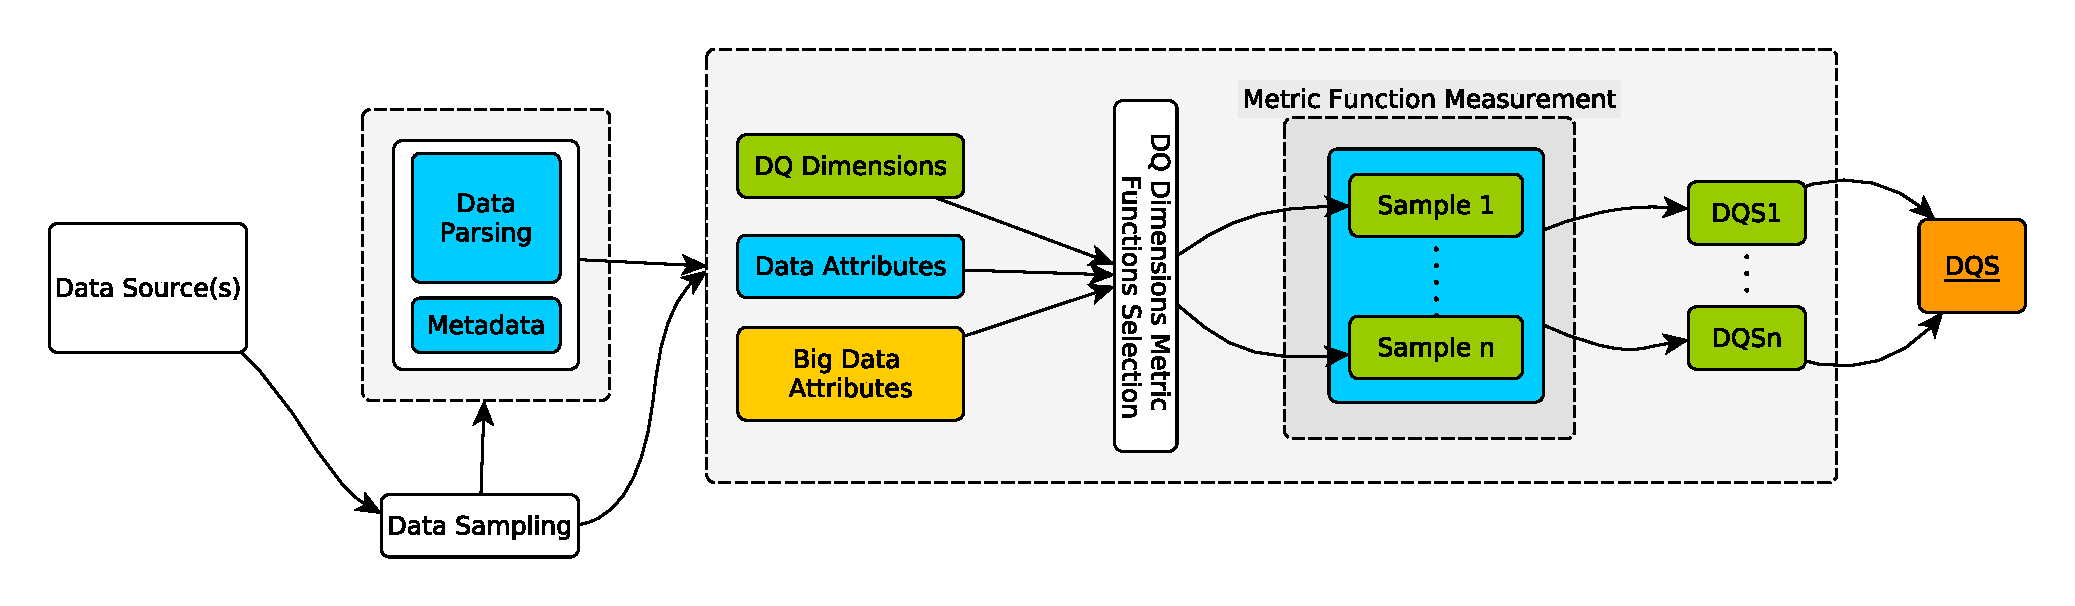
\includegraphics[scale=.55]{big_data_quality_evaluation_scheme}
	\caption{Big Data Quality Evaluation Scheme}    
\end{figure}

\section{Big Data Quality Evaluation Scheme}

The purpose of Big Data Quality Evaluation (BDQ) Scheme is to address the data quality before starting data analytics.
This is done by estimating the quality of data attributes or features by applying a DQD metric to measure the quality characterized by its
accuracy, completeness or/and consistency. The expected result is data quality assessment suggestions indicating the quality 
constraints that will increase or decrease the data quality.

The BDQ Evaluation scheme is illustrated in Figure 3.1 where the data goes through many module to estimate its quality.
The key modules of our scheme consist of: (a) data sampling; and data profiling, (b) DQD vs attributes selection, 
(c) data quality Metric selection, (d) samples data quality evaluation. In the following sections, we describe each module, its input(s), output(s),
and the main functions.

\subsection{Big Data Sampling}

A sample is representative of a whole population. Based on a sample, we make several decision about a population. 
A sample is also called a subgroup. The number of observations or units in a sample is called sample size. 
The number of times a sample is collected is usually referred to as the sampling frequency. In designing a control chart, we must 
specify both of these parameters. ~\cite{Jugulum14}

There are several sampling strategies that can be applied on Big Data as expressed in ~\cite{Asilomar} ~\cite{SIGKDD}.
They evaluated the effect of sampling methods on Big Data and believed that sampling large datasets reduces run time and computational footprint of link 
prediction algorithms though maintaining sufficient prediction performance. In statistic, Bootstrap sampling technique evaluates the sampling distribution of an 
estimator by sampling with replacement from the original sample. In the context of Big Data, Bootstrap sampling has been addressed in many works 
~\cite{Liang2016} ~\cite{Satyanarayana2014}. 
In our data evaluation scheme will used the Bag of Little Bootstrap (BLB) ~\cite{ArXiv12066415}, which combines the results of bootstrapping multiple small subsets of a 
Big data dataset. THe BLB algorithm use an original Big dataset used generate small samples without replacements. 
For each generated sample another set of samples are created by resampling with replacement.

\subsection{Data Profiling}

Data profiling is an exploratory approach to data quality analysis. Statistical approaches are used to reveal 
data usage patterns as well as patterns in the data ~\cite{Osborne2013} ~\cite{Maydanchik2007}. Several tools exist for data quality assessment using data profiling 
and exploratory data analysis. Such tools include Tableau and Talend Open Studio. 

Data profiling module performs screening of data quality
based on statistics and information summary. Since
profiling is meant to discover data characteristics from data sources. It is considered as data assessment process that
provides a first summary of the data quality. Such information include: data format description, different
attributes, their types and values. data constraints (if any),
data range, max and min. More precisely information about
the data are presented in two types; technical and functional. This information can be extracted from the data itself
without any additional representation using it metadata or any descriptive header file, or by parsing the data using any
analysis tools. This task may become very costly in Big Data. To avoid costs generated due the data size we will use
the same sampling process BLB to reduce the data into a representative population sample, in addition to the combination of profiling results.

\subsection{Data Quality Evaluation}

The data profiling provides information about dataset, 

\begin{itemize}
	\item { Data attributes (eg. type format)}
	\item { Data summary (eg. max, min)}
	\item {Big data attributes; size number of sources speed of data generation (eg. data streams)}
	\item {What DQD evaluate.}
\end{itemize}

The previous information's are used to select the appropriate quality metrics functions \textbf{\textit{F}}
to evaluate a data quality dimensions \textbf{\textit{$d_k$}} for an attribute \textbf{\textit{$a_i$}}
with a weight \textbf{\textit{$w_j$}}

In the Fig 3.2 we describe how data quality evaluated using bootstrap sampling for Big data. The process
follows these steps: 

\begin{enumerate}
	\item {Sampling from the data set \textbf{S} \textbf{n} bootstrap sample size of \textbf{ss} size without replacement \textbf{$DS_j$}. }
	\item {Each sample generated from step 1 is sampled into n' samples of size SS with replacements $DS_{ij}$}
	\item {For the Each sample \textbf{$DS_{ij}$} generated in step 2, evaluate the data quality score $Q_{ij}$}	
\end{enumerate}


\begin{figure}[h]
	\vspace*{-.1in}
	\hspace*{-.6in}
	\centering
	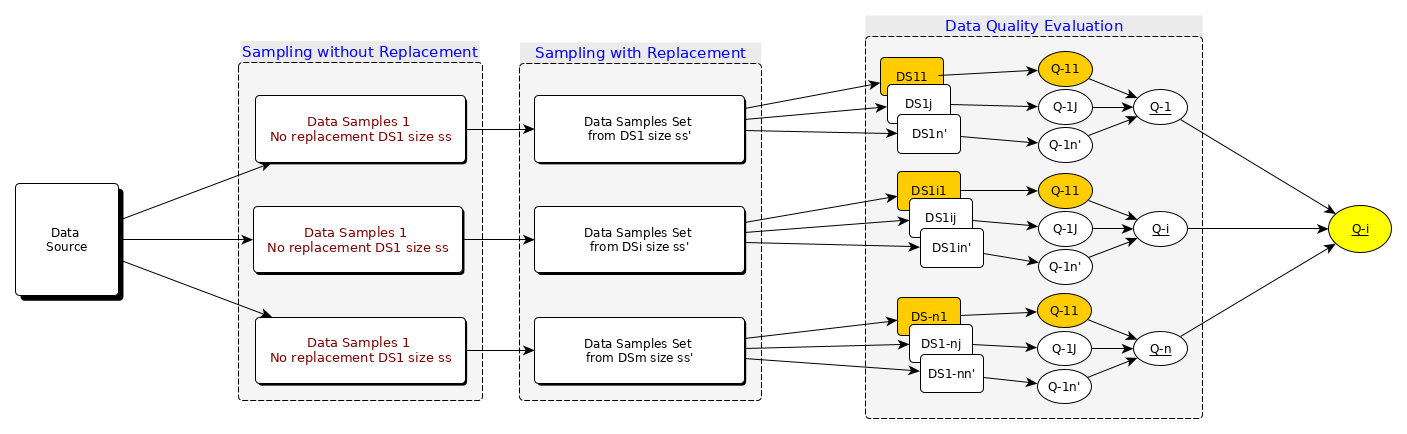
\includegraphics[scale=.38]{big-data-quality-sampling-evaluation}
	\caption{Big Data Quality Sampling Evaluation}    
\end{figure}

\begin{table}[H]
	\caption{Big Data Quality Evaluation Algorithm}
	\centering
	\begin{tabular}{p{15cm}}
	\toprule
	\textbf{Algorithm: Big Data Quality Evaluation} \\ 
	\bottomrule
	\IncMargin{1em}
	\begin{algorithm}[H]
	\SetKwData{Letds}{\textit{\textbf{let ds}}}
	\SetKwData{Letss}{\textit{\textbf{let ss}}}
	\SetKwData{Letn}{\textit{\textbf{let n}}}
	\SetKwData{Letd}{\textit{\textbf{let D}}}
	\SetKwData{Letf}{\textit{\textbf{let F}}}
	\SetKwData{Letcc}{\textit{\textbf{let cc}}}
	\SetKwData{Lets}{\textit{\textbf{let S}}}

	\SetKwData{This}{this}
	\SetKwData{Up}{up}
	\SetKwFunction{Union}{Union}
	\SetKwFunction{MetricFunctionTuple}{MetricFunctionTuple}
	
	
	\SetKwInOut{Input}{input}
	\SetKwInOut{Output}{output}
	
	\Letds a Original Data Set with size \textbf{SS and Observation (N-SS)}\; 
	\Letss  (\textbf{b(SS)}) the samples with ss < SS \;
	\Letn  samples \textbf{$s_i$} of size \textbf{ss} and \textbf{\textit{M}} Observation \textbf{(M-ss)}\;

	\Letd a set of DQD  \textbf{{$D=\{d_0,...d_k,...d_q\}$}}\;
	\Letf a metric function \textbf{F (completeness, accuracy,...)} \;
	\Letcc $\leftarrow$ 0 counter of correct valid attribute value(when \textbf{F} \textit{is true} $cc=cc+1$)\;
	\Lets \textbf{=\{ $DS_0$,...$DS_i$,...$DS_n$  \}} without replacement \;
	\BlankLine

	\For{$i\leftarrow 0$ \KwTo $n$}{
		\emph{Generate sample $s_{i}$ of size SS from ds}\;

		\For{$j\leftarrow 0$ \KwTo $n'$} {

			\emph{Generate a sample $_{ij}$ of size SS from sample $si$}\;

			\For{$k\leftarrow 0$ \KwTo $j$}{
				\MetricFunctionTuple{$d_k,F$} 
				 
				 \For{$a\leftarrow 0$ \KwTo $j$} {

				 	\For{$a_{ij}(x)$ \textbf{ss} values}{ 
						 \If{\textbf{F($a_{ij}(x)$, value) == 1}}{
							\emph{measure metric} \;
							$c\leftarrow$ cc + 1 \; 
							\emph{\textbf{Calculate the scores vector DQD(F, $d_k$,$a_{ij}$, $DS_i$})= $\frac{cc}{N}$}
							$cc\leftarrow$0 \emph{counter of correct valid attribute value \textbf{($d_k$,F)}}
						 }
					 }
					 \emph{DQD $d_k$ computed for all attributes for a sample $ds_{ij}$ }
				 }
				 \emph{$DQS_{ijk}$ is the $D_K$ scores for an attribute $a_ij$ for sample $DS_{ij}$}
				 \emph{$Q_{ijk}$ sum of all $d_k$ scores for attributes $a_{ij}$ for $DS_{ij}$ }
			}
			$Q_{ik} += 1/n'(Q_{ijk})$ 
		 }	
	}
	\emph{$Q_k$ is the mean of all $Q_{ik}$ for a specif $d_k$}
	$Q_k += 1/n(Q_{ik})$
\end{algorithm}\DecMargin{1em}
\\
\end{tabular}
\end{table}


%%!TEX root = ../thesis.tex
%*******************************************************************************
%****************************** Forth Chapter **********************************
%*******************************************************************************
\chapter{Experimentations , Results and Analysis}

% **************************** Define Graphics Path **************************
\ifpdf
    \graphicspath{{Chapter4/Figs/Raster/}{Chapter4/Figs/PDF/}{Chapter4/Figs/}}
\else
    \graphicspath{{Chapter4/Figs/Vector/}{Chapter4/Figs/}}
\fi

In this chapter, we will explain how data quality dimensions are implemented with Machine Learning (ML) techniques towards dirty datasets. 

\section{Experimental Methodology}  

The impact of the dirt data and data cleaning on ML in a dataset depends on a number of factors -- some factors depend on the data cleaning process, 

i.e., the error types to be cleaned and the cleaning methods; some factors depend on the ML
process, i.e., the model types used; and some factors depend on where the cleaning is performed during the ML process. Hence, in order to comprehensively investigate the impacts, we need to consider data cleaning an ML jointly in our experiments.


\section{The NettoyageML \cite{Nettoyage2019} Schema}  

The NettoyageML relational schema consists of three relations as shown in Table ~\ref{table:nettoyage_ml} . Firstly will introduced the attributes of NettoyageML relational models, and then will explained 
the differences between these three relations.


\begin{itemize}
	\item {
		\textbf{Attributes for Dataset.} The first attribute is dataset, which is the input to the data cleaning and ML pipeline. Each dataset can have multiply types of errors and has an associated ML task. 
	}
\end{itemize}


\begin{table}[H]
	\label{table:nettoyage_ml}
		
	\leftskip=3em
	\begin{flushleft}
		\leftskip=3em
		\textbf{R1 Vanilla}
	\end{flushleft}
	\begin{tabular}{|c|c|c|c|c|c|c|}
		\hline 
		Dataset & Error Type & Detection & Repair & ML Model & Scenario & Flag \\ 
		\hline 
	\end{tabular} \linebreak	

	\begin{flushleft}
		\leftskip=3em
		\textbf{R2 (With Model Section)}
	\end{flushleft}
	\begin{tabular}{|c|c|c|c|c|c|c|}
		\hline 
		Dataset & Error Type & Detection & Repair & Scenario & Flag \\ 
		\hline 
	\end{tabular} \linebreak

	\begin{flushleft}
		\leftskip=3em
		\textbf{R3 (With Model Selection and Cleaning Method Selection)}
	\end{flushleft}	

	\begin{tabular}{|c|c|c|c|c|c|c|}
		\hline 
		Dataset & Error Type & Scenario & Flag \\ 
		\hline 
	\end{tabular} \linebreak
	\caption{NettoyageML Relational Schema}
\end{table}

Even for one error type, they might appear in a dataset in various distributions and hence affect ML models in complicated ways







%\include{Chapter5/chapter5}
%\include{Chapter6/chapter6}
%\include{Chapter7/chapter7}



% ********************************** Back Matter *******************************
% Backmatter should be commented out, if you are using appendices after References
%\backmatter

% ********************************** Bibliography ******************************
\begin{spacing}{0.9}

% To use the conventional natbib style referencing
% Bibliography style previews: http://nodonn.tipido.net/bibstyle.php
% Reference styles: http://sites.stat.psu.edu/~surajit/present/bib.htm

\bibliographystyle{apalike}
%\bibliographystyle{unsrt} % Use for unsorted references  
%\bibliographystyle{plainnat} % use this to have URLs listed in References
\cleardoublepage
\bibliography{References/references} % Path to your References.bib file


% If you would like to use BibLaTeX for your references, pass `custombib' as
% an option in the document class. The location of 'reference.bib' should be
% specified in the preamble.tex file in the custombib section.
% Comment out the lines related to natbib above and uncomment the following line.

%\printbibliography[heading=bibintoc, title={References}]


\end{spacing}

% ********************************** Appendices ********************************

\begin{appendices} % Using appendices environment for more functunality

%!TEX root = ../thesis.tex
% ******************************* Thesis Appendix A ****************************
\chapter{How to use NettoyageML} 

\begin{flushleft}
	This is the EISTI.NettoyageML Benchmark for Joint Data Cleaning and Machine Learning. 
	The codebase is located in: \url{https://github.com/aytacozkan/EISTI.NettoyageML}
\end{flushleft}

\section{Basic Usage}

\subsection*{Run Experiments}

\begin{flushleft}
	To run experiments, download and unzip the 
	\href{https://drive.google.com/file/d/1BdLZAyp5KSvj8AdL2by9bNkRxX8po1FL/view?usp=sharing}{datasets}. 
	Place it under the project home directory and execute the following command from the project home directory:
\end{flushleft}


\begin{lstlisting}[language=python]
		python3 main.py --run_experiments [--dataset <name>] \
		\[--cpu <num_cpu>][--log]
\end{lstlisting}

\subsubsection*{Options}

\begin{itemize}
	\item {
		\textbf{--dataset:} the experiment dataset. If not specified, the program will run experiments on all datasets.
	}
	\item {
		\textbf{--cpu:} the number of cpu used for experiment. Default is 1.
	}
	\item {
	\textbf{--log:} whether to log experiment process.
	}
\end{itemize}


\subsubsection*{Output}

The experimental results for each dataset will be saved in `/result` directory as a json file named as <dataset name>\_result.json. Each result is a key-value pair. The key is a string in format "<dataset><split seed><error type><clean method><ML model><random search seed>". The value is a set of key-value pairs for each evaluation metric and result. Our experimental results are provided in `result.zip`.


\subsection*{Run Analysis}
To run analysis for populating relations described in the paper, unzip \textbf{`result.zip`} and execute the following command from the project home directory:

\begin{lstlisting}[language=python]
		python3 main.py --run_analysis [--alpha <value>]
\end{lstlisting}

\subsubsection*{Options}

\begin{itemize}
	\item {
	\textbf{--alpha:} the significance level for multiple hypothesis test. Default is 0.05.	
}
\end{itemize}


\subsubsection*{Output}
The relations R1, R2 and R3 will be saved in \textbf{`/analysis`} directory. Our analysis results are provided in `analysis.zip`.


\section{Extend Domain of Attributes}

\subsection*{Add new datasets}

To add a new dataset, first, create a new folder with dataset name under \textbf{`/data`} and create a `raw` folder under the new folder.  The `raw` folder must contain raw data named \textbf{`raw.csv`}. For dataset with inconsistencies, it must also contain the inconsistency-cleaned version data named \textbf{`inconsistency\_clean\_raw.csv`}. For dataset with mislabels, it must also contain the mislabel-cleaned version data named \textbf{`mislabel\_clean\_raw.csv`}. The structure of the directory looks like:


\dirtree{%
	.1 /.
	.2 data.
	.3 new\_dataset.
	.4 raw.
	.5 raw.csv.
	.5 inconsistency\_clean\_raw.csv (for dataset with inconsistencies).
	.5 mislabel\_clean\_raw.csv (for dataset with mislabels).
}

Then add a dictionary to \textbf{`/schema/dataset.py`} and append it to \textbf{`datasets`} array at the end of the file.

The new dictionary must contain the following keys:

\begin{lstlisting}[language=xml]
data_dir: the name of the dataset.
error_types: a list of error types that the dataset contains.
label: the label of ML task.
\end{lstlisting}

The following keys are optional:

\begin{lstlisting}[language=xml]
class_imbalance: whether the dataset is class imbalanced.
categorical_variables: a list of categorical attributes.
text_variables: a list of text attributes.
key_columns: a list of key columns used for deduplication.
drop_variables: a list of irrelevant attributes.
\end{lstlisting}

\subsection*{Add new error types}
To add a new error type, add a dictionary to `/schema/error\_type.py` and append it to `error\_types` array at the end of the file.

The new dictionary must contain the following keys:

\begin{lstlisting}[language=xml]
name: the name of the error type.
cleaning_methods: a dictionary, {cleaning method name: cleaning methods object}.
\end{lstlisting}

\subsection*{Add new models}
To add a new ML model, add a dictionary to `/schema/model.py` and append it to `models` array at the end of the file.

The new dictionary must contain the following keys:

\begin{lstlisting}[language=xml]
name: the name of the model.
fn: the function of the model.
fixed_params: parameters not to be tuned.
hyperparams: the hyperparameter to be tuned.
hyperparams_type: the type of hyperparameter "real" or "int".
hyperparams_range: range of search. Use log base for real type hyperparameters.
\end{lstlisting}


\subsection*{Add new cleaning methods}
\begin{flushleft}
	To add a new cleaning methods, add a class to `/schema/cleaning\_method.py`.

The class must contain two methods:
\end{flushleft}

\textbf{`fit(dataset, dirty\_train)`:} take in the dataset dictionary and dirty training set. Compute statistics or train models on training set for data cleaning.

\textbf{`clean(dirty\_train, dirty\_test)`}: take in the dirty training set and dirty test set. Clean the error in the training set and test set. Return \textbf{`(clean\_train, indicator\_train, clean\_test, indicator\_test)`}, which are the clean version datasets and indicators that indicate the location of error. 

\subsection*{Add new scenarios}
We consider "BD" and "CD" scenarios in our paper. To investigate other scenarios, add scenarios to `/schema/scenario.py`.


%!TEX root = ../thesis.tex
% ******************************* Thesis Appendix B ********************************

\chapter{Installing the CUED class file}

\LaTeX.cls files can be accessed system-wide when they are placed in the
<texmf>/tex/latex directory, where <texmf> is the root directory of the user’s \TeX installation. On systems that have a local texmf tree (<texmflocal>), which
may be named ``texmf-local'' or ``localtexmf'', it may be advisable to install packages in <texmflocal>, rather than <texmf> as the contents of the former, unlike that of the latter, are preserved after the \LaTeX system is reinstalled and/or upgraded.

It is recommended that the user create a subdirectory <texmf>/tex/latex/CUED for all CUED related \LaTeX class and package files. On some \LaTeX systems, the directory look-up tables will need to be refreshed after making additions or deletions to the system files. For \TeX Live systems this is accomplished via executing ``texhash'' as root. MIK\TeX users can run ``initexmf -u'' to accomplish the same thing.

Users not willing or able to install the files system-wide can install them in their personal directories, but will then have to provide the path (full or relative) in addition to the filename when referring to them in \LaTeX.



\end{appendices}

% *************************************** Index ********************************
\printthesisindex % If index is present

\end{document}
